% !TEX root = ../report.tex

\chapter{The SoBazaar Data}
\label{sobazaar-data}
\minitoc

    This sections will introduce the SoBazaar application and explore the SoBazaar data set.
    This includes how the data was preprocessed, a summary of the dataset, statistics and graphs about the data and findings from the data.

	\section{The SoBazaar Application}\mbox{}\\

	\begin{chapquote}[30pt]{About SoBazaar}
	  "SOBAZAAR is a newly developed social shopping experience – a daily fashion bazaar on your mobile."
	\end{chapquote}

	SoBazaar is an online marketplace for fashion, but with a social twist. The application lets you click through thousands of products. You can find stores like Moods of Norway, BIK BOK, Bianco and many more. If you find something you like you can purchase it directly from the application or store it for later with the \emph{love it} functionality.
	The following screenshots are taken from the application and highlights some functionality currently found in the
	application.

	\begin{figure}[H]
		\centering
		\begin{minipage}{.30\linewidth}
	  		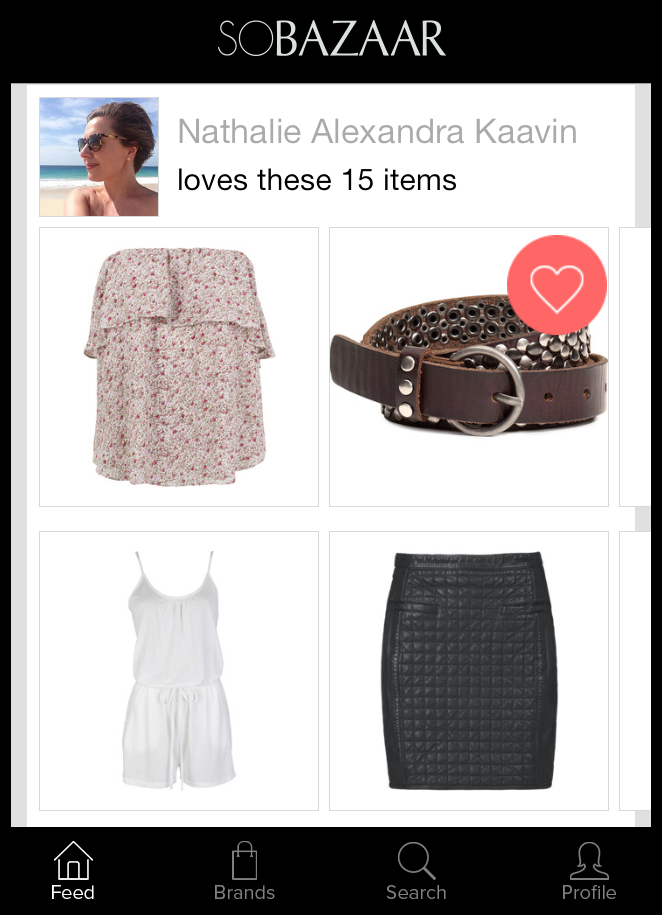
\includegraphics[height=1.5\linewidth]{image/SoBazaarfeed.png}
		\end{minipage}
		\hspace{.02\linewidth}
		\begin{minipage}{.30\linewidth}
			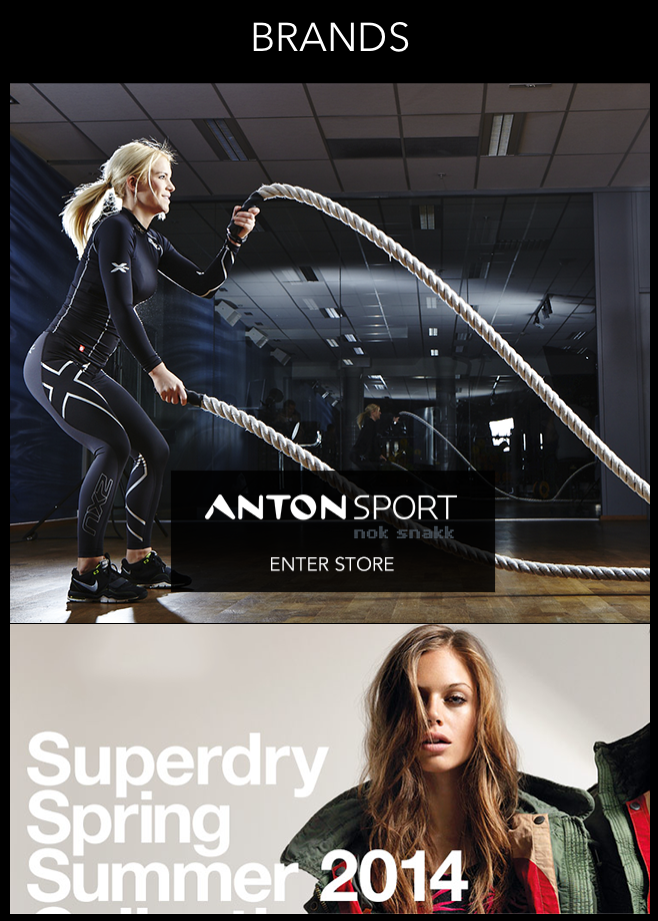
\includegraphics[height=1.5\linewidth]{image/SoBazaarbrands2.png}
		\end{minipage}
		\hspace{.02\linewidth}
		\begin{minipage}{.30\linewidth}
			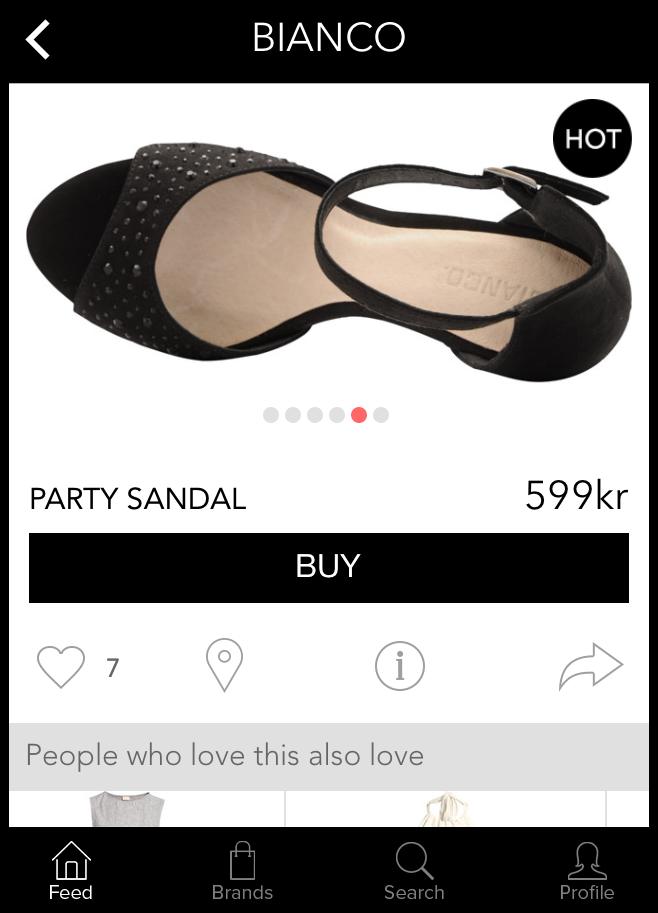
\includegraphics[height=1.5\linewidth]{image/SoBazaarproduct.png}
		\end{minipage}
		\caption[SoBazaar screenshots - version 0.5.1]{Screenshots from the SoBazaar Application. From the left to right: The SoBazaar newsfeed, the brand browser screen and the product detail screen}
		\label{figure:SoBazaarfeed}
	\end{figure}

	To help the customers find products the feed currently shows the activity of other users, notifies you about sales,
	presents the most popular items and the application also features an editors pick page among other things.
	The following screenshots show some functionality currently in place to help the customer find items to buy.

	\begin{figure}[H]
		\centering
		\begin{minipage}{.3\linewidth}
		  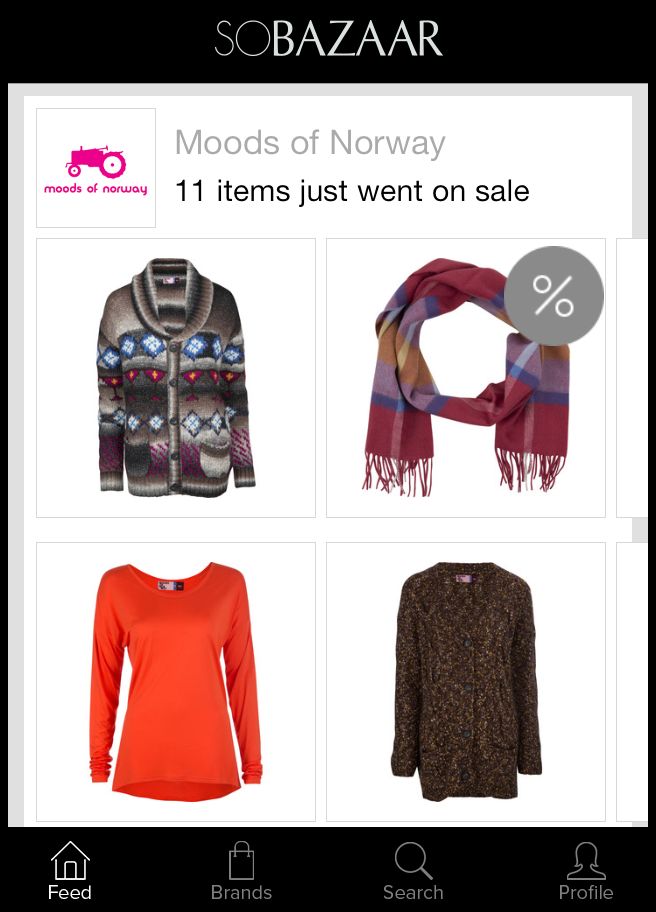
\includegraphics[height=1.5\linewidth]{image/SoBazaarsale.png}
		\end{minipage}
		\hspace{.02\linewidth}
		\begin{minipage}{.3\linewidth}
		  
\includegraphics[height=1.5\linewidth]{image/SoBazaareditor.png}
		\end{minipage}
		\hspace{.02\linewidth}
		\begin{minipage}{.3\linewidth}
			  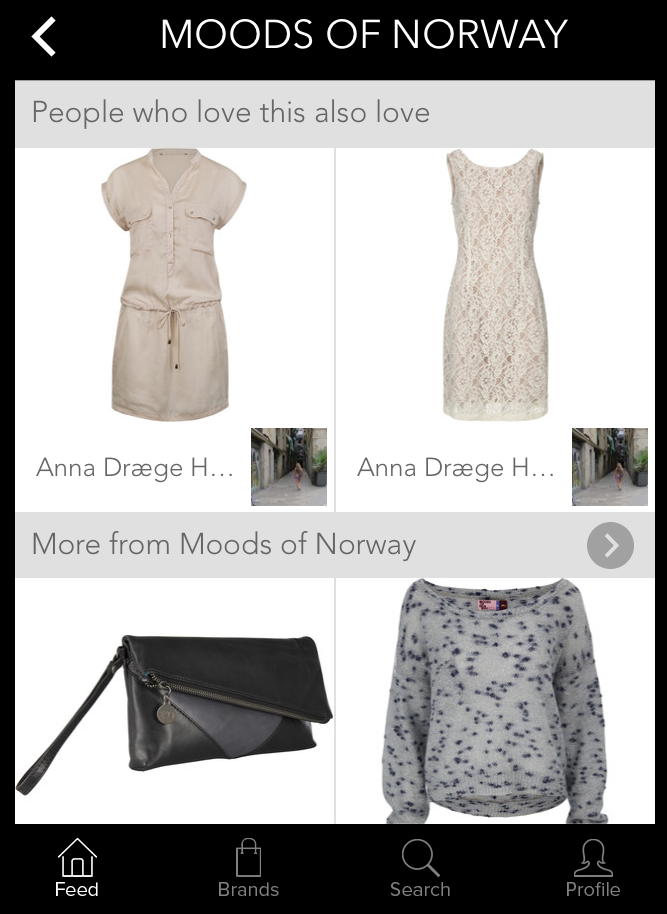
\includegraphics[height=1.5\linewidth]{image/SoBazaarrelated.png}
		\end{minipage}
		\caption[SoBazaar screenshots - version 0.5.1]{Screenshots from the SoBazaar Application. From the left to right: A newsfeed sale notification, editors picks and related product widgets from the product screen}
		\label{figure:SoBazaarfeed}
	\end{figure}

	The application is currently in a beta phase and is planned for a final release after the summer.

% mtodo - før vi kan lære dette
    % 2. sessions of events m eksempel

\section{Preprocessing}
    The data from SoBazaar came as is from the SoBazaar database, with the exception that the data had been anonymised for privacy reasons.
    It therefore contained some unwanted events, such as automated queries producing unnatural spikes of events on items and events with missing fields.
    The data was therefore cleaned by removing events containing test environment flags such as: test environment and applications run from simulator.
    What was left after the cleaning data was mainly events triggered by the users, and not created during applications testing.

\section{Dataset Summary}
    The data from SoBazaar is gathered based on the actions of the users in the application.
    When a user accesses a store or an item, the information regarding the user and the item is stored, this is often known as implicit feedback~\ref{sec:implicit}.
    Events such as purchasing an item and "wanting" and item is stored in the same manner, but can in many cases be considered as explicit feedback.

    When an event is triggered a set of information is stored regarding the event.
    This data is used to make recommendations for the users though converting the implicit feedback to implicit ratings.

    \begin{table}[H]
        \centering
        \begin{tabular}{l l}
            \toprule
            Variable     & Explanation   \\ \midrule
            price             & The price of the item which triggered the event \\
            product\_id       & The id of the item which triggered the event \\
            storefront\_id    & The store id from which the item originated \\
            event\_id         & What kind of event was triggered~\tablefootnote{Complete list of the different types of events can be found in table~\ref{table:events}} \\
            event\_location   & The location of the user when the event was triggered \\
            ts                & Unix timestamp in milliseconds of when the event was triggered \\
            session           & Which session number the event belongs too~\tablefootnote{This value is added at a later time. For two events to end up in the same session, the event has to be triggered within a certain period of time, and both be after the same application started-flag} \\
            user\_id          & The unique id of the user who triggered the event \\
            \bottomrule
        \end{tabular}
        \label{table:eventData}
        \caption[Event Metadata]{Metadata collected from an event. The complete list can be found in table~\ref{table:completeEventData}}
    \end{table}

    \begin{table}[H]
        \centering
        \begin{tabular}{l l}
            \toprule
            Attribute       & Count   \\ \midrule
            Total number of events  &    218975 \\
            Unique users ids    &    2021 \\
            Unique item ids     &    6092 \\
            Unique storefronts  &    147 \\
            Unique brands   &    24 \\
            Item clicks     &    25491 \\
            Item wants   &    13262 \\
            Item purchases   &    2020 \\
            Average item click count per user   &    12.6130 \\
            Average purchase count per user     &    6.5620 \\
            Average rating per user     &    19.6889 \\
            Average rating per item     &    6.6796 \\
            \bottomrule
        \caption[Dataset summary]{Overview of the key figures in the SoBazaar dataset}
        \label{table:datasetSummary}
        \end{tabular}
    \end{table}
    \marginpar{input the updated data when/if we get a new dump from SoBazaar}

\section{Graphs}
    % Price range of items in stores
    % user-item (how many items has a user "interacted" with)
    % Count of unique items in item db also in event db
    % Usable events regarding userid (events types with not null userid)
    % unique Stores count for users
    %     price span for user
    %         Timespann of sessions for users (avg, max, min)
    %         Events per session (avg, max, min)
    %         Item viewtime for user in session
    %         Stores visited per session
    %         revisit time of items for user
    %         relationship with view, want and purchase
    %         time of session over lifetime of app
    %         user preferred price in session
    %         price vs view, want and purchase
    %         avg viewtime for an item (i know)
    %         Similarity of user favorite store, items viewed and items wanted?
    %         time of session over lifetime of app for all users (slope-style)
    % new:
    %     item timespan (first item interest - last item interest)
    % User stats: items, likes, intented purchased, events, session avg, max event, fequency

\subsection{User properties}
    \begin{figure}[H]
        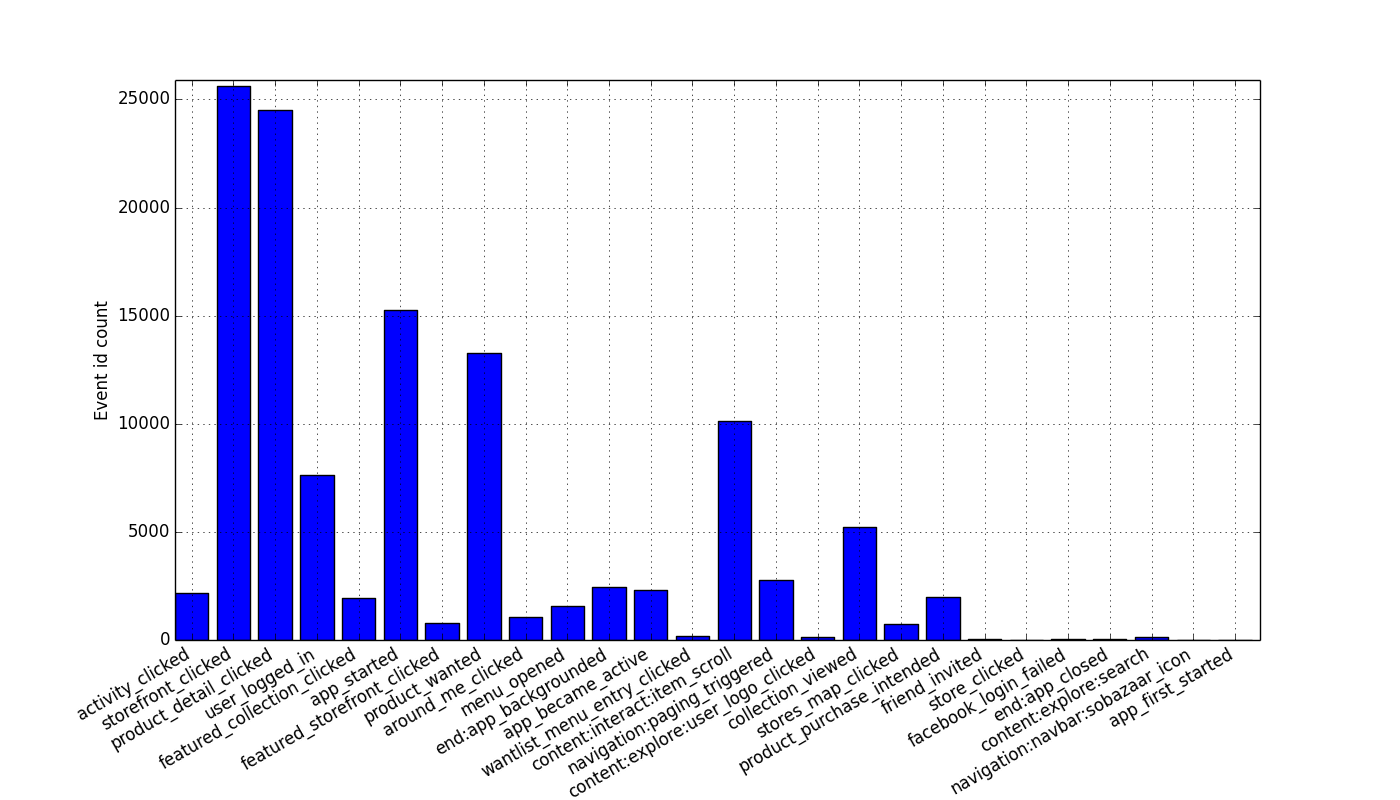
\includegraphics[width=5in]{image/event_iddistribution.png}
        \centering
        \caption{Count for different events}
    \label{figure:eventIDDistribution}
    \end{figure}
        This figure displays the count for each of the different events which can be triggered in the SoBazaar application.
        The "collection\_viewed"-event and "storefront\_clicked"-event are the most common events to be triggered.
        Both of these types of events will send the user to an item overview, and indicates that many users browse the items through looking at the thumbnails rather than accessing the items, since the two named event types are gateways to collections of items, and if most of the users actually accessed most of the items the "product\_detail\_clicked", "product\_wanted" and "product\_purchase\_intended" would have had the majority of the events triggered.

    \begin{figure}[H]
        \centering
        \begin{subfigure}{.5\textwidth}
            \centering
            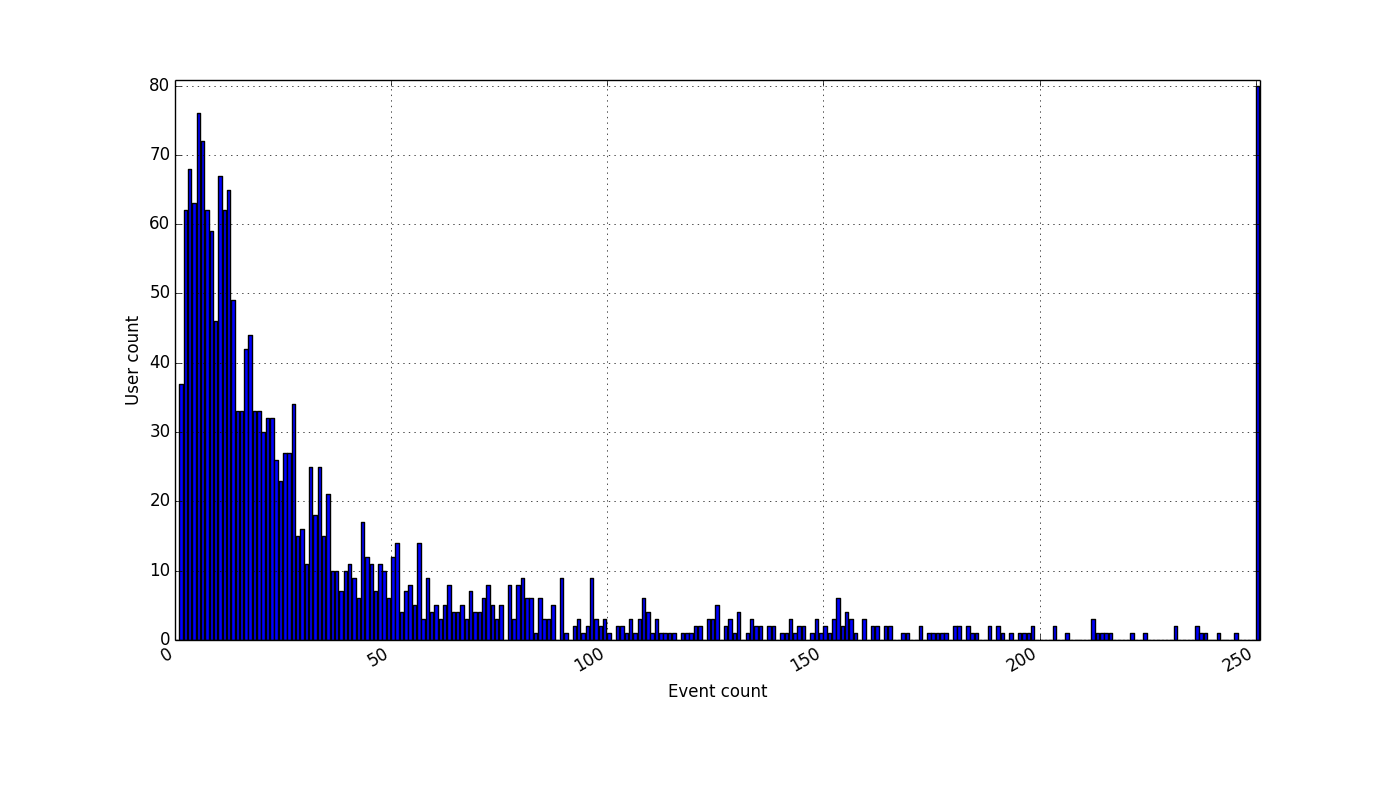
\includegraphics[width=\dualGraphWidth]{image/user_iddistribution.png}
            \caption{mtodo}
    \label{figure:userEventDist}
        \end{subfigure}%
        \begin{subfigure}{.5\textwidth}
            \centering
            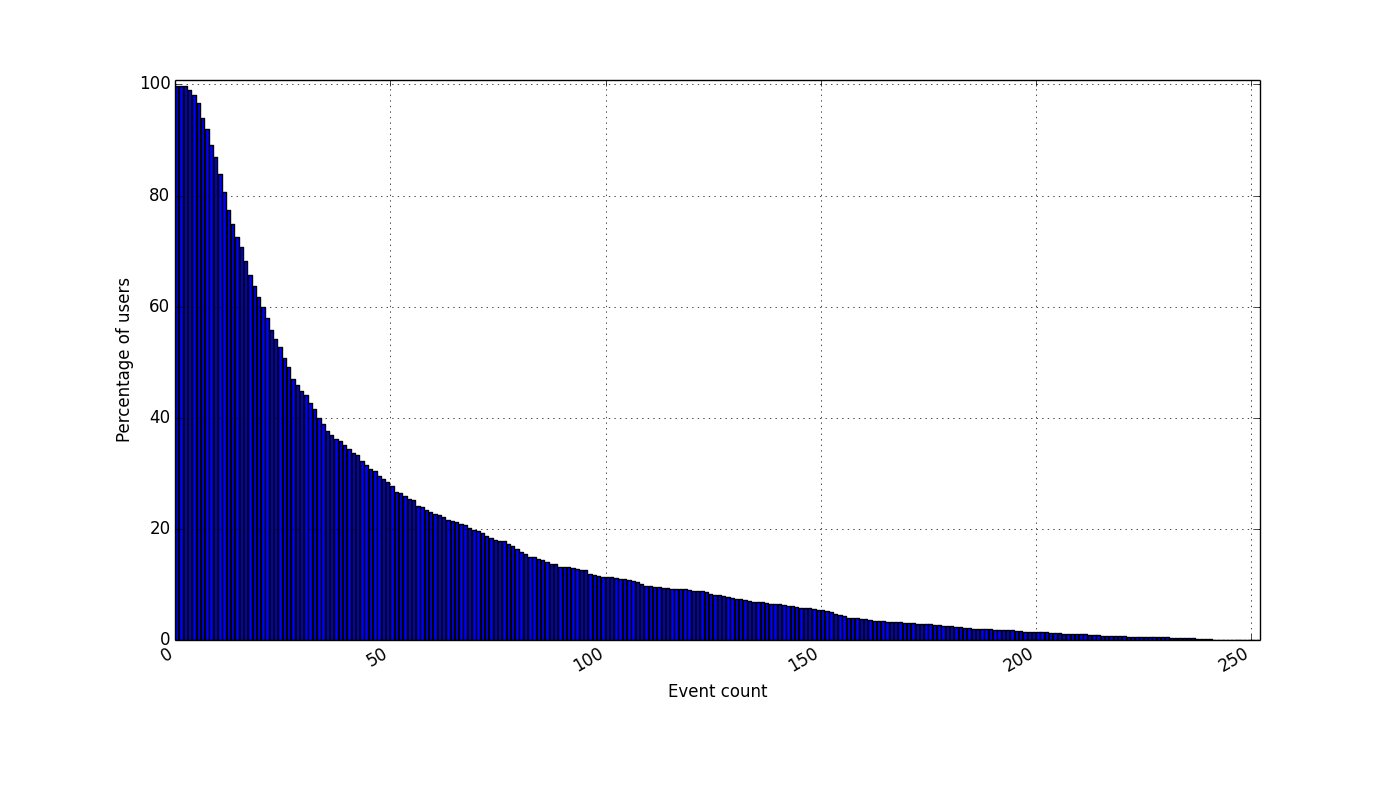
\includegraphics[width=\dualGraphWidth]{image/user_idcumdistribution.png}
            \caption{mtodo}
    \label{figure:userEventCumDist}
        \end{subfigure}
        %
    \end{figure}

    \begin{figure}[H]
        \centering
        \begin{subfigure}{.5\textwidth}
            \centering
            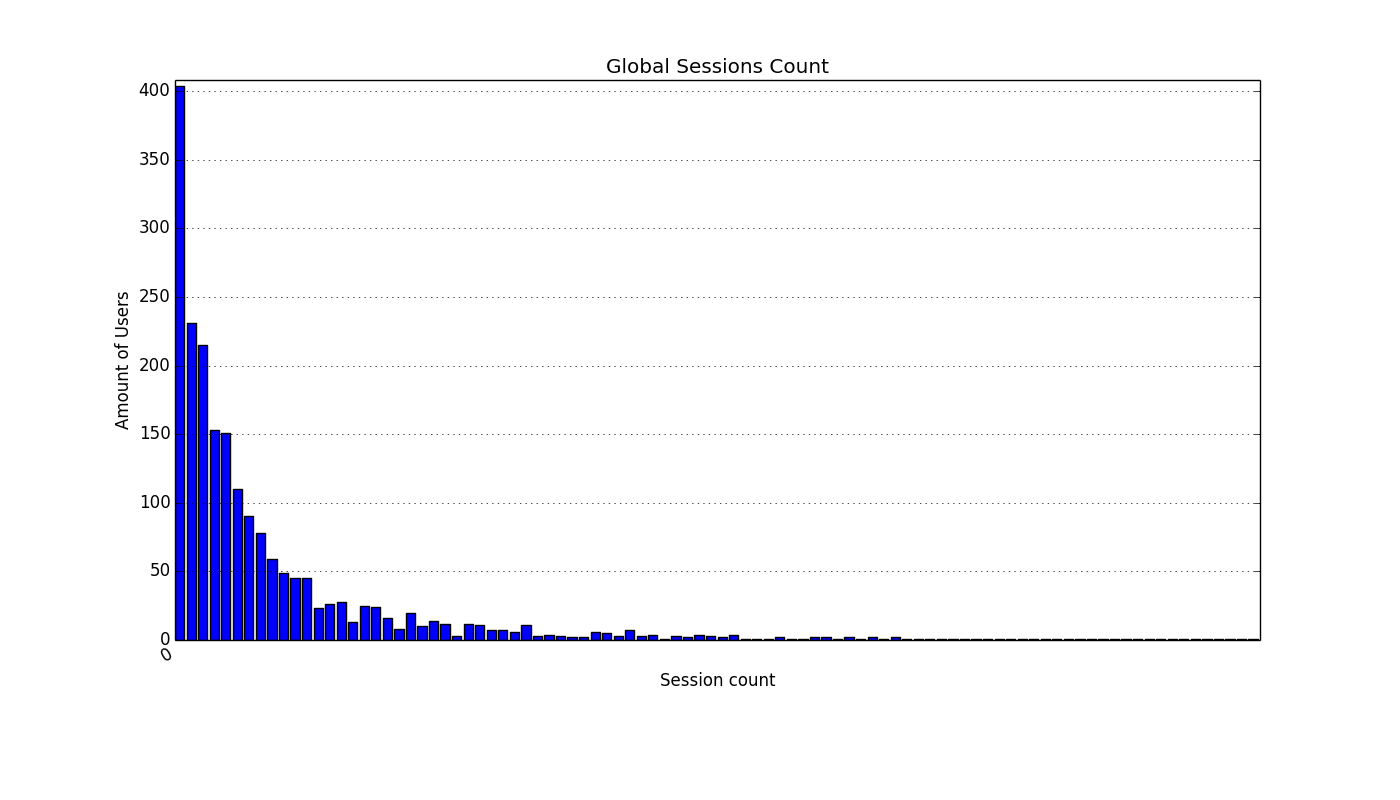
\includegraphics[width=\dualGraphWidth]{image/sessionsCountdistribution.png}
            \caption{Distribution of sessions for users}
    \label{figure:sessCountDist}
        \end{subfigure}%
        \begin{subfigure}{.5\textwidth}
            \centering
            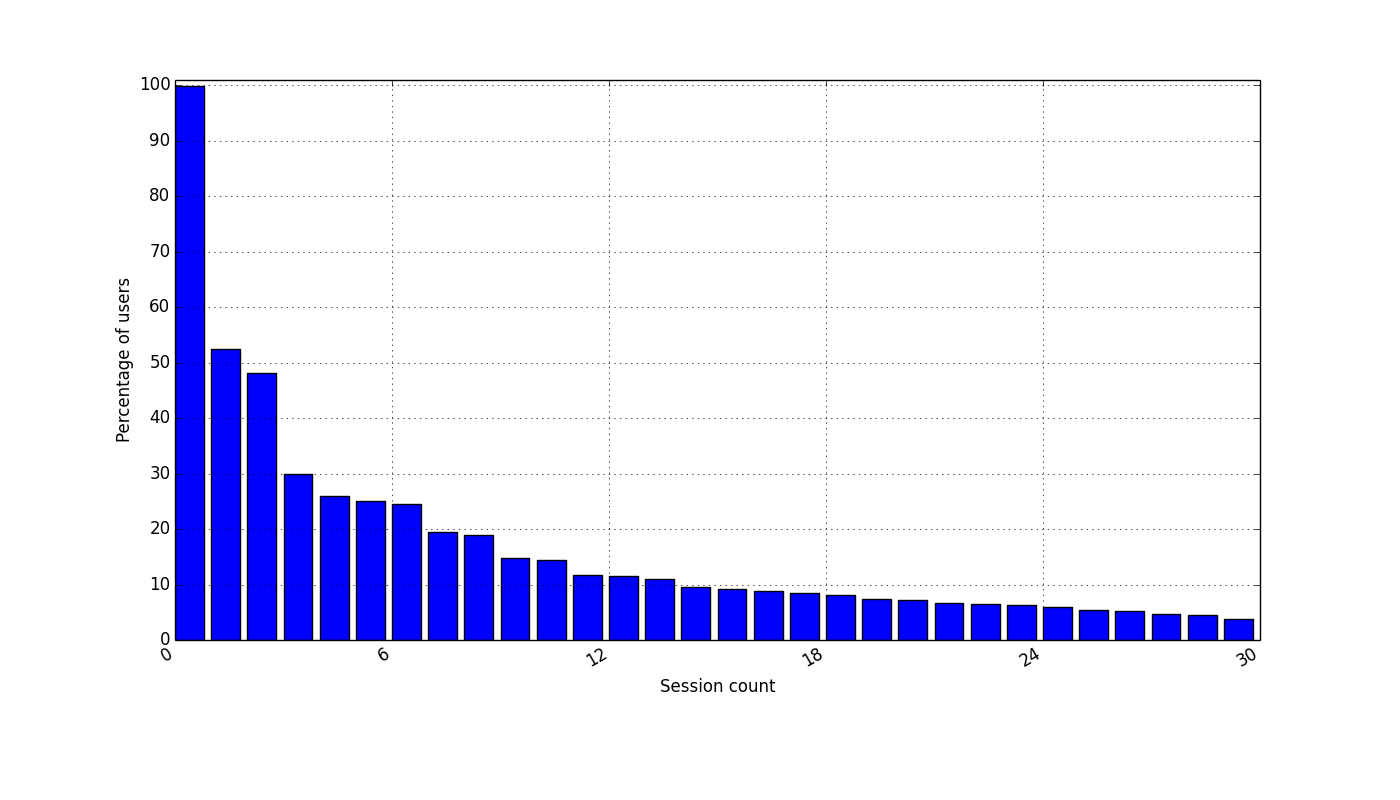
\includegraphics[width=\dualGraphWidth]{image/sessioncumdistribution.png}
            \caption{View times before purchasing an item}
    \label{figure:sessCountCumDist}
        \end{subfigure}
        %
    \end{figure}
        The maximum number of sessions for each user grouped to show how the count of how many users has the different amount of sessions.
        The majority of the users of SoBazaar has a session count of 20 and less.
        This means that they have not used the applications more than 20 separate times, over the time the data was collected.


    \begin{figure}[H]
        \centering
        \begin{subfigure}{.5\textwidth}
            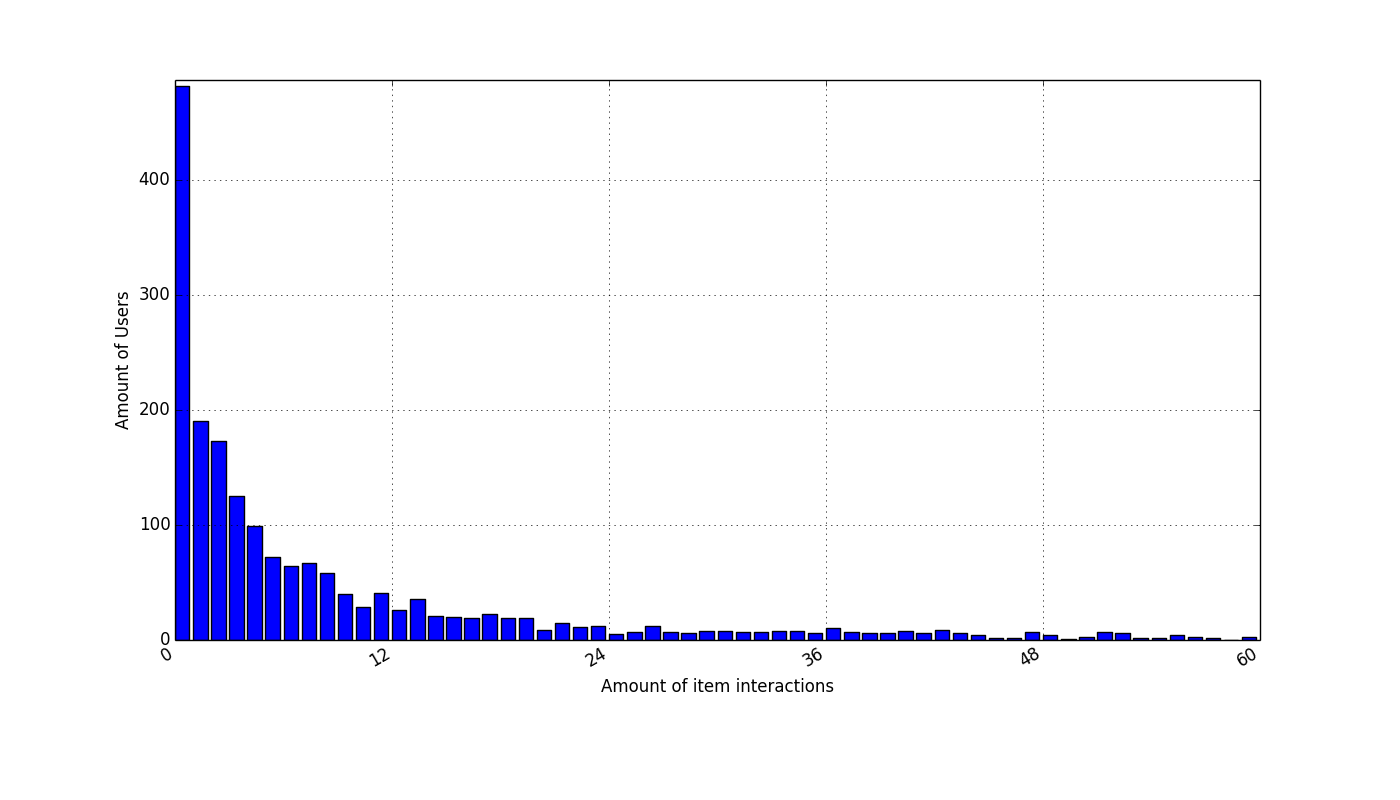
\includegraphics[width=\dualGraphWidth]{image/ratingsPerUserdistribution.png}
            \centering
            \caption{Count of ratings for users}
    \label{figure:ratingsPerUser}
        \end{subfigure}%
        \begin{subfigure}{.5\textwidth}
            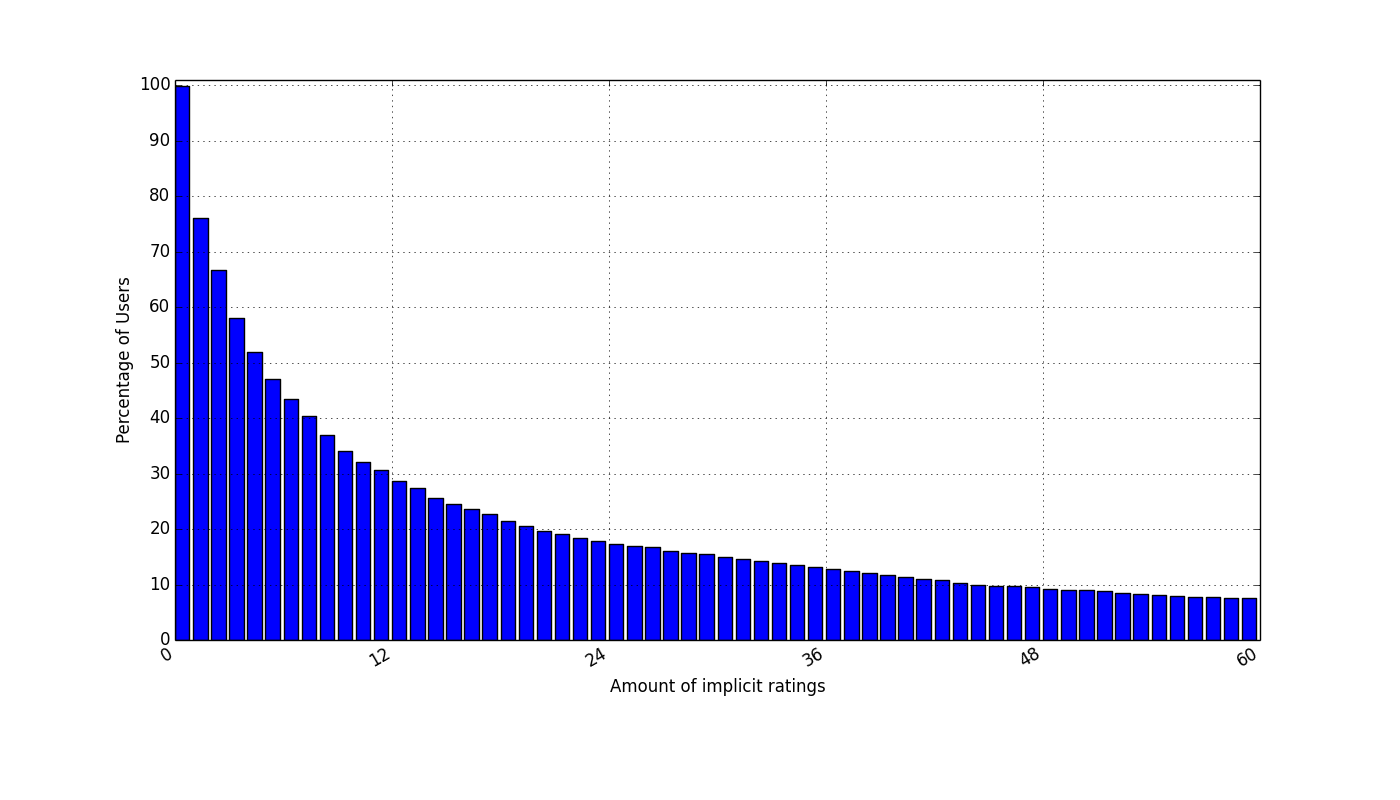
\includegraphics[width=\dualGraphWidth]{image/ratingsPerUsercumdistribution.png}
            \centering
            \caption{Cumulative count of ratings for users}
    \label{figure:ratingsPerUserCum}
        \end{subfigure}
        %
    \end{figure}


    \begin{figure}[H]
        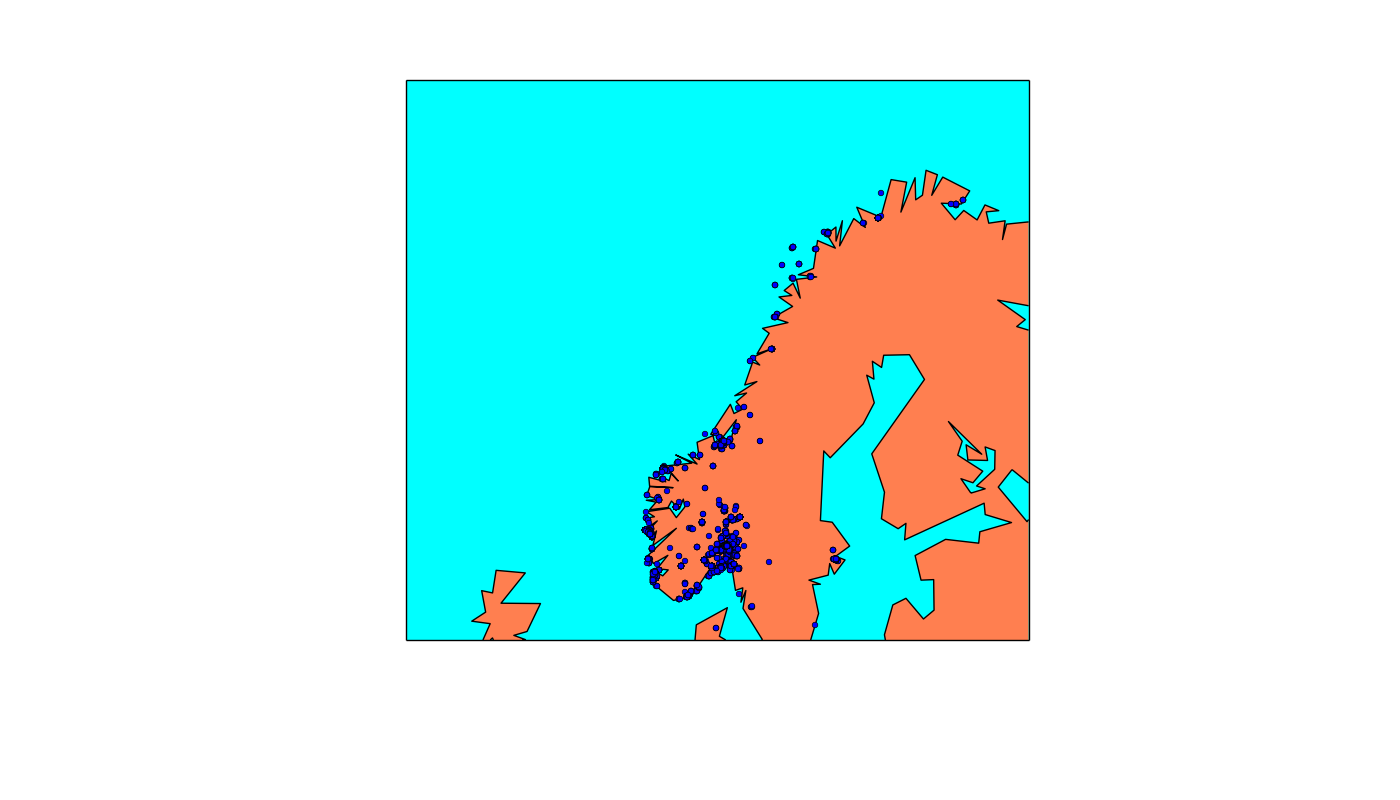
\includegraphics[width=5in]{image/simpleGeoPlotNorway.png}
        \centering
        \caption{Simple plotting of event location}
    \label{figure:croppedGeoplot}
    \end{figure}
        This figure shows the location of the user at the time of the different event triggers.
        It is cropped to show events triggered in and around Norway.
        We can see that the majority of the users are located in and around Oslo.

\subsection{Product properties}

    \begin{figure}[H]
        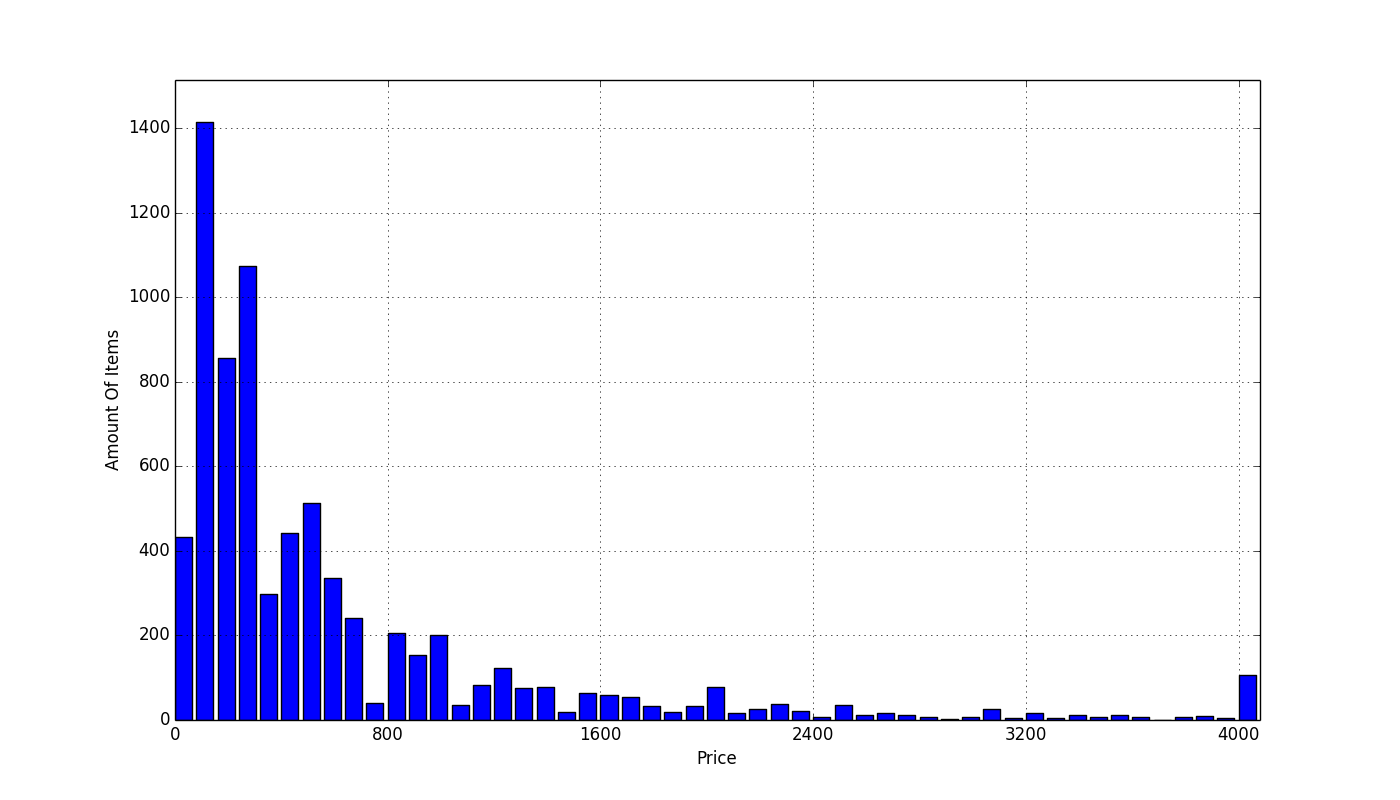
\includegraphics[width=5in]{image/priceDistribution.png}
        \centering
        \caption{Price distribution of items}
    \label{figure:priceDistribution}
    \end{figure}
        Here we see how them items are distributed on amount of items and price. The red bars indicates the amount of items with the belonging price.
        All items priced over 3 000 are put in the same bucket, and is the reason for the last spike we see at 3 000.
        We can see from this graph that the majority of the items are priced under 1 000 NOK.

    \begin{figure}[H]
        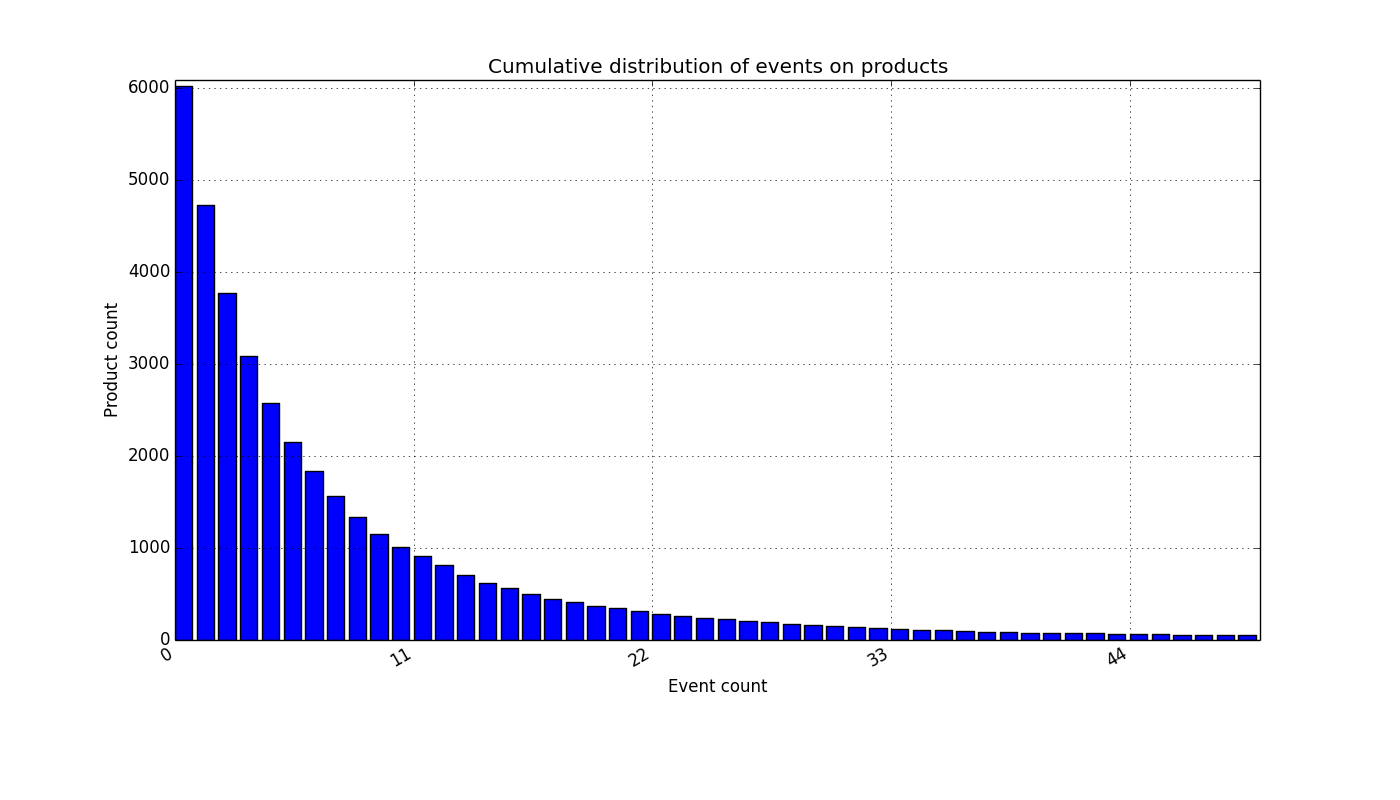
\includegraphics[width=5in]{image/product_idcumdistribution.png}
        \centering
        \caption{Count of events on each unique item}
    \label{figure:eventOnProductDist}
    \end{figure}
        This figure shows the unique count of events on each item in the SoBazaar dataset.
        The majority of the items has only had a interaction count of 10 or less.
        Interaction count is "product\_detail\_clicked", "product\_wanted" and "product\_purchase\_intended".
        This means that there will not be more than 10 events for the majority of the items, which might lead to an issue when doing collaborative filtering on the data.
        When the majority of the events only has 10 events and there are over 4 000 items and 1 200 users, the probability that multiple users have interacted with similar items will be low.

\subsubsection{Long tail and the Pareto principle}

    For a given distribution such as sales of a catalog of items, when the Pareto principle applies, the first 20\% of the item hits account for 80\% of sales.

    or

    Long tail: the most frequent-occurring items represent less than 50\% of the occurrences in the logs. ~\cite{DBLP:journals/corr/abs-1203-4487}


    \begin{figure}[H]
        \centering
        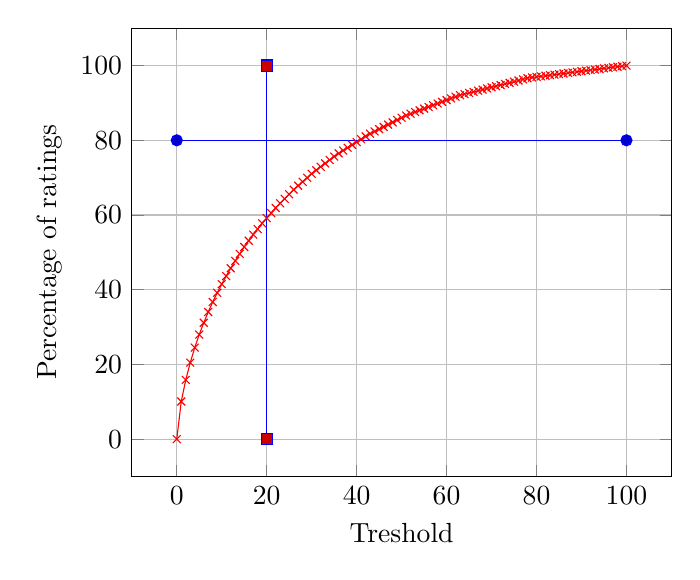
\begin{tikzpicture}
            \begin{axis}[
                xlabel=Treshold,
                ylabel=Percentage of ratings,
                grid=major,
            ]
            \addplot+[color=blue,sharp plot] coordinates
                {(0,80) (100,80)};
            \addplot+[color=blue,sharp plot] coordinates
                {(20,0) (20,100)};
            \addplot[color=red,mark=x] coordinates {
                    (0.0, 0.0)
                    (1.0, 10.089827139370456)
                    (2.0, 15.879525954256096)
                    (3.0, 20.48914274211811)
                    (4.0, 24.52004126512845)
                    (5.0, 28.004931686083083)
                    (6.0, 31.16775281181592)
                    (7.0, 34.053795636967514)
                    (8.0, 36.72848048712981)
                    (9.0, 39.184258863196035)
                    (10.0, 41.49409958986488)
                    (11.0, 43.66303499987419)
                    (12.0, 45.76151775155373)
                    (13.0, 47.72412751931158)
                    (14.0, 49.60370379689505)
                    (15.0, 51.44553757894472)
                    (16.0, 53.116272047907806)
                    (17.0, 54.75178018770601)
                    (18.0, 56.2614800090582)
                    (19.0, 57.79634149409959)
                    (20.0, 59.17016833153008)
                    (21.0, 60.52889817074705)
                    (22.0, 61.887628009964025)
                    (23.0, 63.14571119442417)
                    (24.0, 64.35347105150593)
                    (25.0, 65.56123090858767)
                    (26.0, 66.78912009662079)
                    (27.0, 67.84842613793623)
                    (28.0, 68.90521601288278)
                    (29.0, 69.9620058878293)
                    (30.0, 71.03640892735828)
                    (31.0, 72.00261681302368)
                    (32.0, 72.90843670583499)
                    (33.0, 73.8142565986463)
                    (34.0, 74.73517348967114)
                    (35.0, 75.64099338248245)
                    (36.0, 76.49900611428427)
                    (37.0, 77.25385602496037)
                    (38.0, 78.02128676748107)
                    (39.0, 78.77613667815716)
                    (40.0, 79.53098658883326)
                    (41.0, 80.29841733135395)
                    (42.0, 81.05326724203005)
                    (43.0, 81.77540698991017)
                    (44.0, 82.37928691845104)
                    (45.0, 82.9932315124676)
                    (46.0, 83.59711144100848)
                    (47.0, 84.20099136954934)
                    (48.0, 84.80487129809023)
                    (49.0, 85.41881589210678)
                    (50.0, 86.02269582064767)
                    (51.0, 86.62657574918853)
                    (52.0, 87.11974435749693)
                    (53.0, 87.57265430390258)
                    (54.0, 88.02556425030824)
                    (55.0, 88.47847419671389)
                    (56.0, 88.9389326422263)
                    (57.0, 89.39184258863196)
                    (58.0, 89.84475253503761)
                    (59.0, 90.29766248144327)
                    (60.0, 90.75812092695568)
                    (61.0, 91.21103087336134)
                    (62.0, 91.66394081976699)
                    (63.0, 92.06149510605641)
                    (64.0, 92.36343507032684)
                    (65.0, 92.66537503459729)
                    (66.0, 92.96731499886772)
                    (67.0, 93.27428729587601)
                    (68.0, 93.57622726014644)
                    (69.0, 93.87816722441687)
                    (70.0, 94.18010718868732)
                    (71.0, 94.48707948569559)
                    (72.0, 94.78901944996603)
                    (73.0, 95.09095941423647)
                    (74.0, 95.39289937850691)
                    (75.0, 95.69987167551518)
                    (76.0, 96.00181163978563)
                    (77.0, 96.30375160405606)
                    (78.0, 96.61072390106435)
                    (79.0, 96.8170495433158)
                    (80.0, 96.96801952545103)
                    (81.0, 97.11898950758624)
                    (82.0, 97.27247565609038)
                    (83.0, 97.4234456382256)
                    (84.0, 97.57441562036082)
                    (85.0, 97.72538560249603)
                    (86.0, 97.87887175100018)
                    (87.0, 98.0298417331354)
                    (88.0, 98.18081171527061)
                    (89.0, 98.33429786377475)
                    (90.0, 98.48526784590997)
                    (91.0, 98.6362378280452)
                    (92.0, 98.7872078101804)
                    (93.0, 98.94069395868455)
                    (94.0, 99.09166394081976)
                    (95.0, 99.24263392295498)
                    (96.0, 99.3936039050902)
                    (97.0, 99.54709005359435)
                    (98.0, 99.69806003572957)
                    (99.0, 99.84903001786478)
                    (100.0, 100.0)
            };
            \end{axis}
        \end{tikzpicture}
        \caption{Pareto's principle values graphed}
    \label{figure:paretosPrinciple}
    \end{figure}

    \begin{table}[H]
        \centering
        \begin{tabular}{lll}
        \toprule
        Threshold &   Cut at~\tablefootnote{Cut top down} &      Percentage of ratings \\
        \midrule
        20.0    &    1206   &    59.1701 \\
        40.0    &    2411   &    79.5309 \\
        50.0    &    3014   &    86.0226 \\
        \bottomrule
        \end{tabular}
        \caption{Pareto's principle values}
    \label{table:paretosPrinciple}
    \end{table}

    \begin{table}[H]
        \centering
        \begin{tabular}{llll}
        \toprule
        Average rating count   & Cut at~\tablefootnote{Cut from bottom and up}  & Coverage & Percentage of ratings \\
        \midrule
        6.5941   &    1833   & 69.5868 &   28.5408 \\
        \bottomrule
        \end{tabular}
        \caption{Long tail values}
    \label{table:longtail}
    \end{table}


    % mtodo - price for store dist
    \begin{figure}[H]
        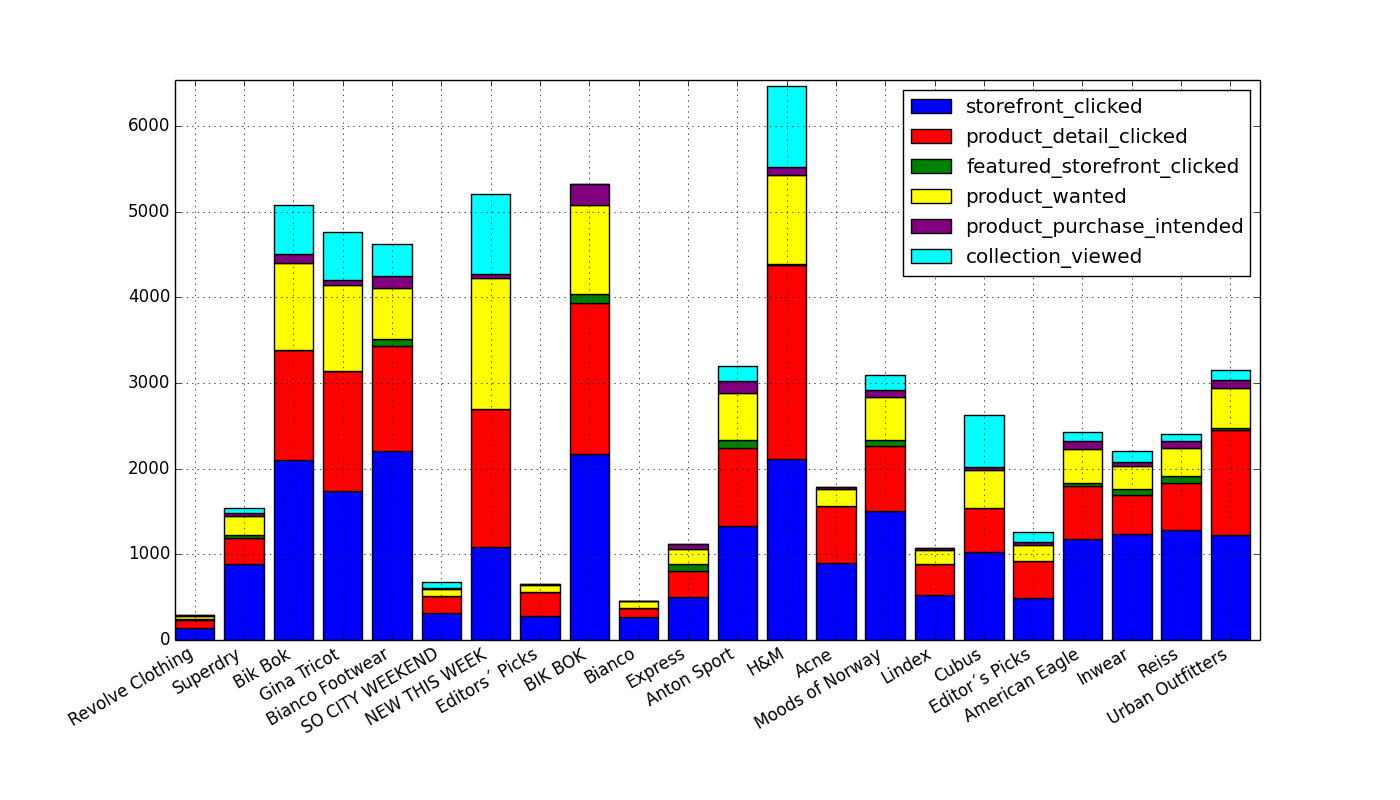
\includegraphics[width=5in]{image/storefront_nameandEventdistribution.png}
        \centering
        \caption{Distribution of events on storefronts}
    \label{figure:eventOnStoreFrontDist}
    \end{figure}
        The events triggered in context with the different storefronts.
        The events are segmented to show the different event counts on the different storefronts, and stacked to show the complete count, to be able to clearly see how the events are distributed over the different stores.
        We can see that "Bik Bok" is the most popular store on all fields.
        One interesting find to take from this graph is the "storefront\_clicked" to the item interaction related events ("product\_detail\_clicked", "product\_wanted" and "product\_purchase\_intended") ratio.
        For instance "Bik Bok" has a much higher item interaction count than storefront access count, whereas stores such as "Reiss" and "Inwear" are mostly accessed and the items not interacted with.
        Different aspects affecting this might be price, style and item presentation.

    \begin{figure}[H]
        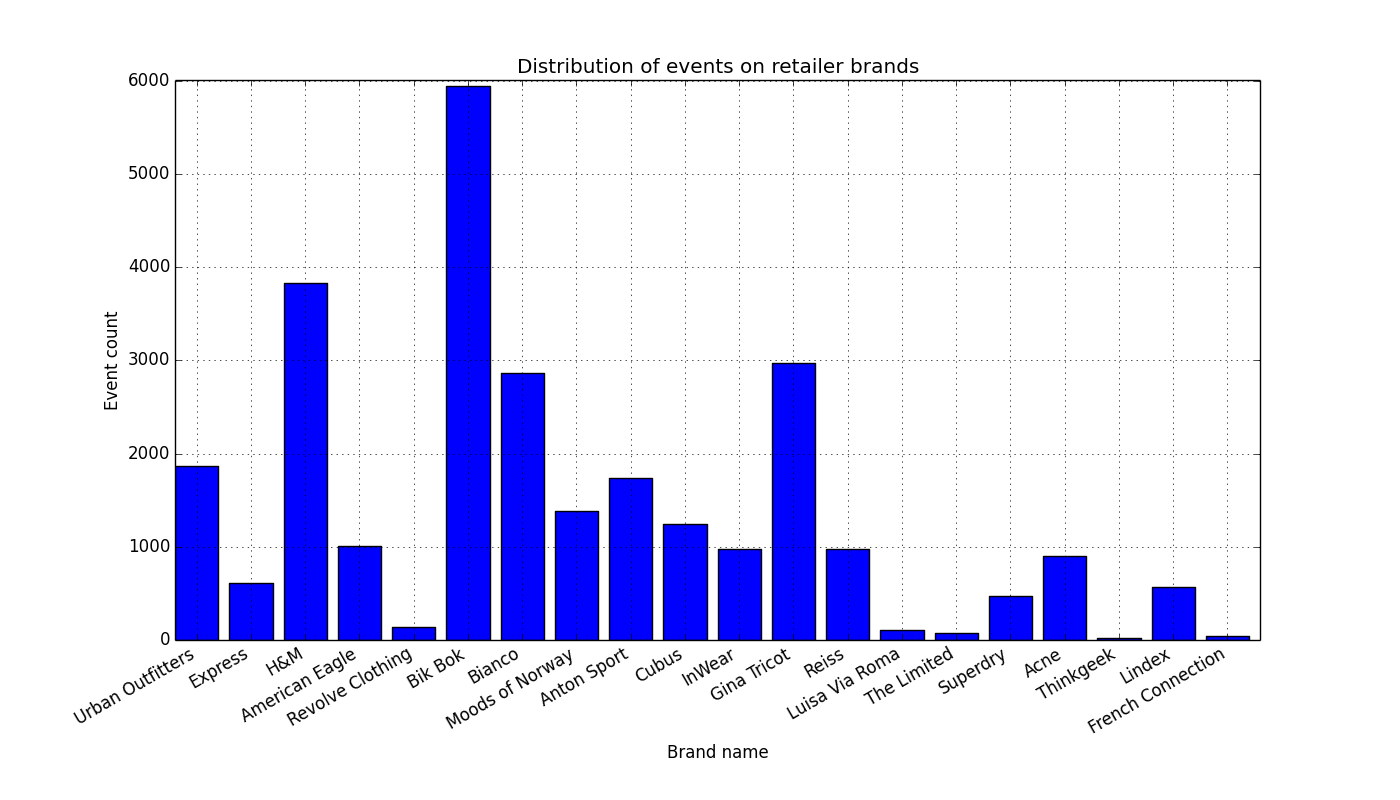
\includegraphics[width=5in]{image/retailer_branddistribution.png}
        \centering
        \caption{mtodo}
    \label{figure:retailerBDist}
    \end{figure}


\subsection{Time properties}

    \marginpar{First to last event in days/weeks not minutes, remove text on a-axis (only confusing). Why is this important, clearify text, what can we learn from the plots?}
    % mtodo - si noe om hvorfor ikke? jeg vil vel påstå at dette sier no om viktihet av "nyhetsverdi" for item'et, og ville derfor trodd dette var relevant info?
    % mtodo - fix while watching AT wooo
    \begin{figure}[H]
        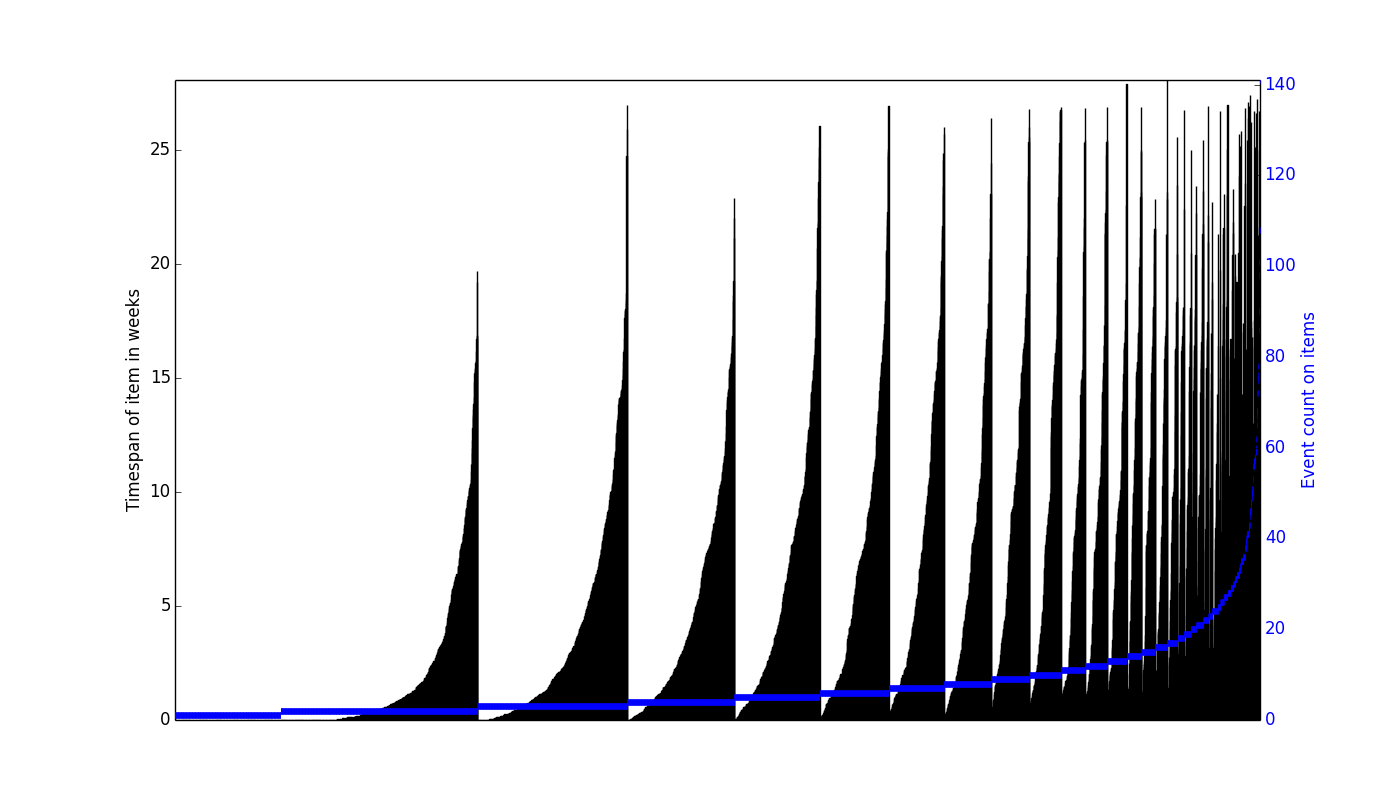
\includegraphics[width=5in]{image/itemTimeSpansortedoneventcount.png}
        \centering
        \caption[Life time of items mapped with event count]{}
    \label{figure:itemTimeSpanEventCount}
    \end{figure}
        This figure shows the total life span of each item mapped together with the amount of events triggered on them.
        The life span of an item is the time since the first event on the item till the last event on the item.
        Time is shown in minutes, so the longest time span of an item is about 105 days, which is close to the time span of the events gathered from SoBazaar.
        Even though an item has had a long time span does not mean that the item has been of measurable interest to the users in the SoBazaar application.

    \marginpar{TODO: Change x axis from minutes to days (or preferably weeks). Does this give us any hints regarding time decay factors?}
    \begin{figure}[H]
        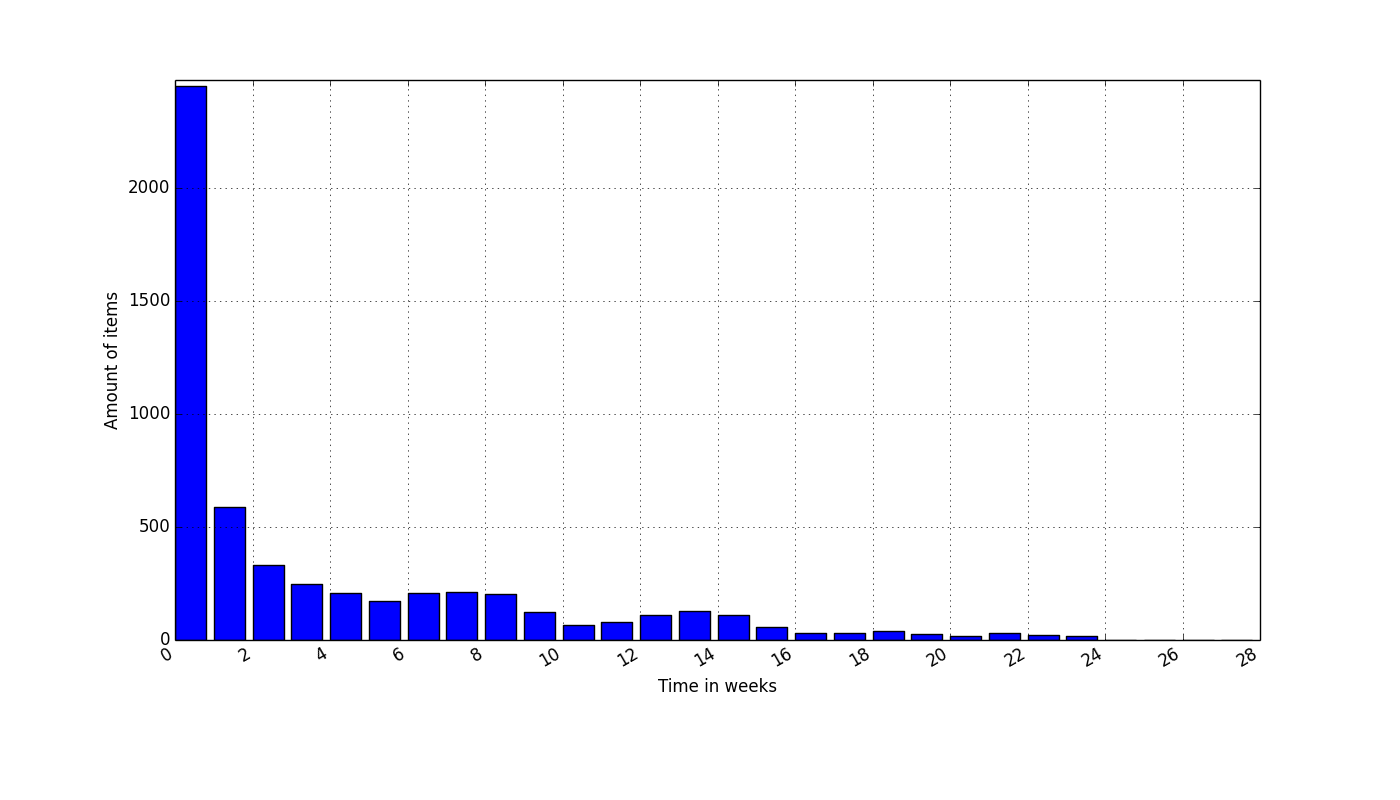
\includegraphics[width=5in]{image/itemTimespansdistribution.png}
        \centering
        \caption{Count of the different time spans of the items}
    \label{figure:itemLifes}
    \end{figure}
        This figure shows the count of items which has the different time spans.
        The numbers on the x-axis is in minutes.
        This figure makes it clearer than figure~\ref{figure:itemTimeSpanEventCount} how long the majority of the the items have lived.
        Most of the items has a time span of less than 14 000 minutes, which is less than 10 days.

    % hvorfor? er det pga:
        % a) pga veldig få events
        % b) pga kort levetid for item i datasettet
        % c) fordi det bare hadde 10 dagers "nyhetsverdi"?
    \begin{figure}[H]
        \centering
        \begin{subfigure}{.5\textwidth}
            \centering
            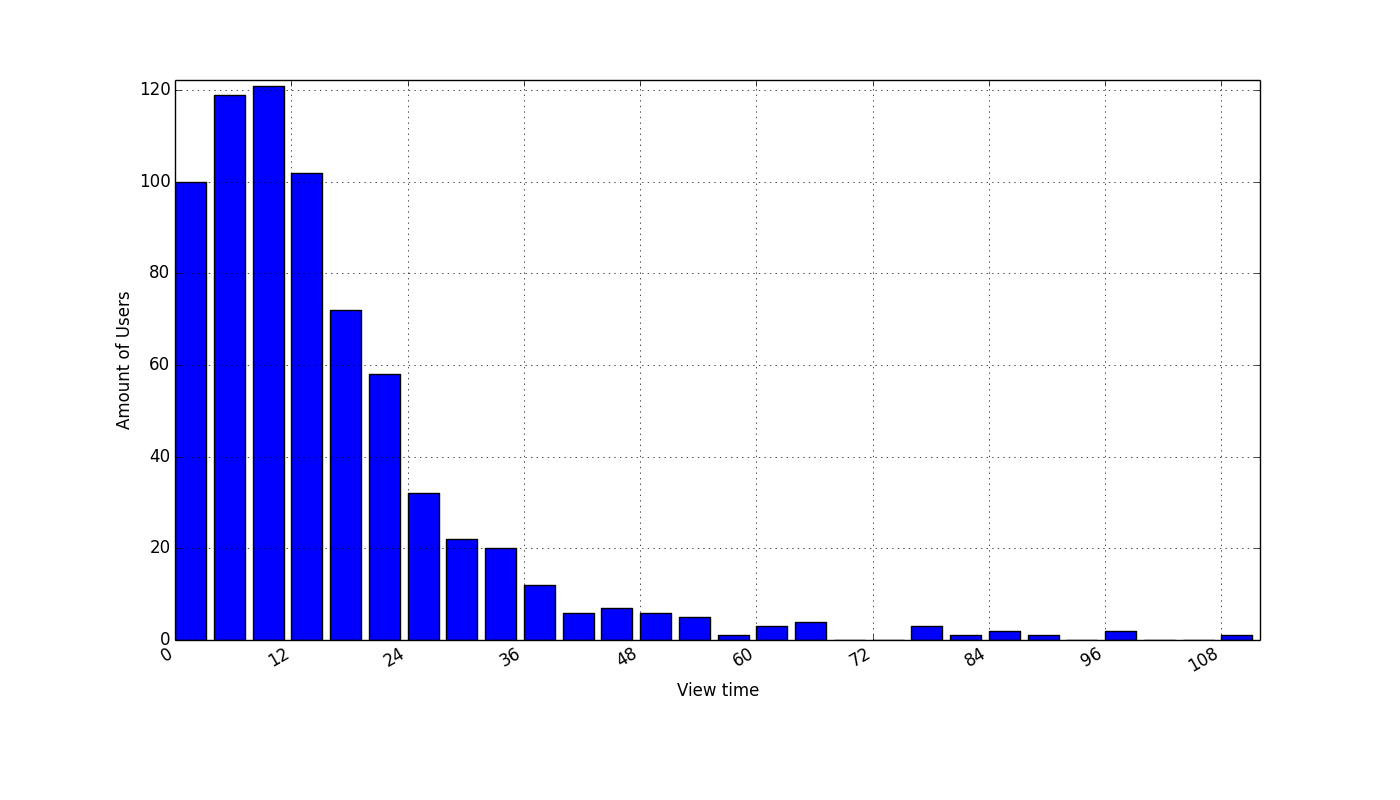
\includegraphics[width=\dualGraphWidth]{image/product_wanteddistribution.png}
            \caption{View times before wanting an item}
    \label{figure:viewWant}
        \end{subfigure}%
        \begin{subfigure}{.5\textwidth}
            \centering
            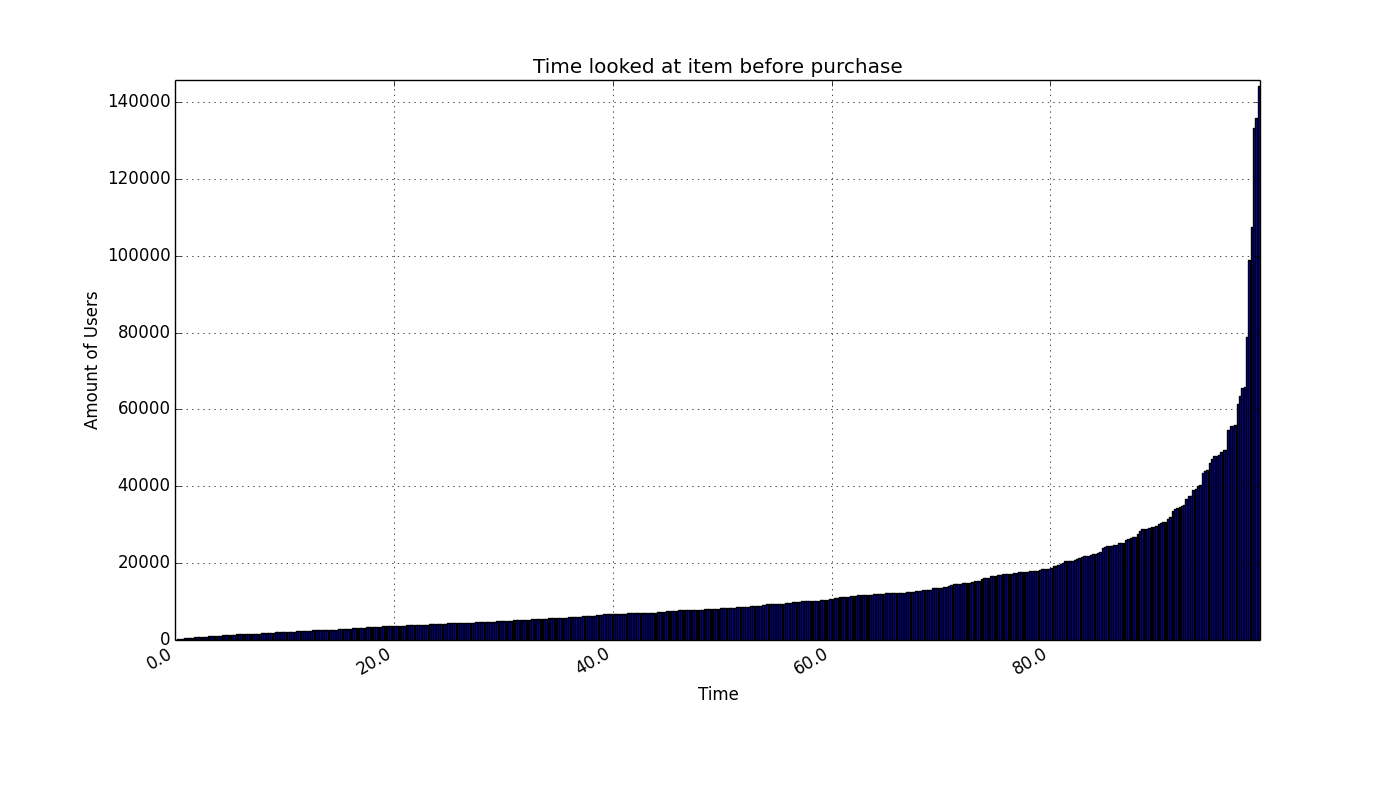
\includegraphics[width=\dualGraphWidth]{image/product_purchase_intendeddistribution.png}
            \caption{View times before purchasing an item}
    \label{figure:viewBuy}
        \end{subfigure}
        %
    \end{figure}

    % mtodo - hva betyr dette for oss? ha det i seconds, lol
    \begin{figure}[H]
        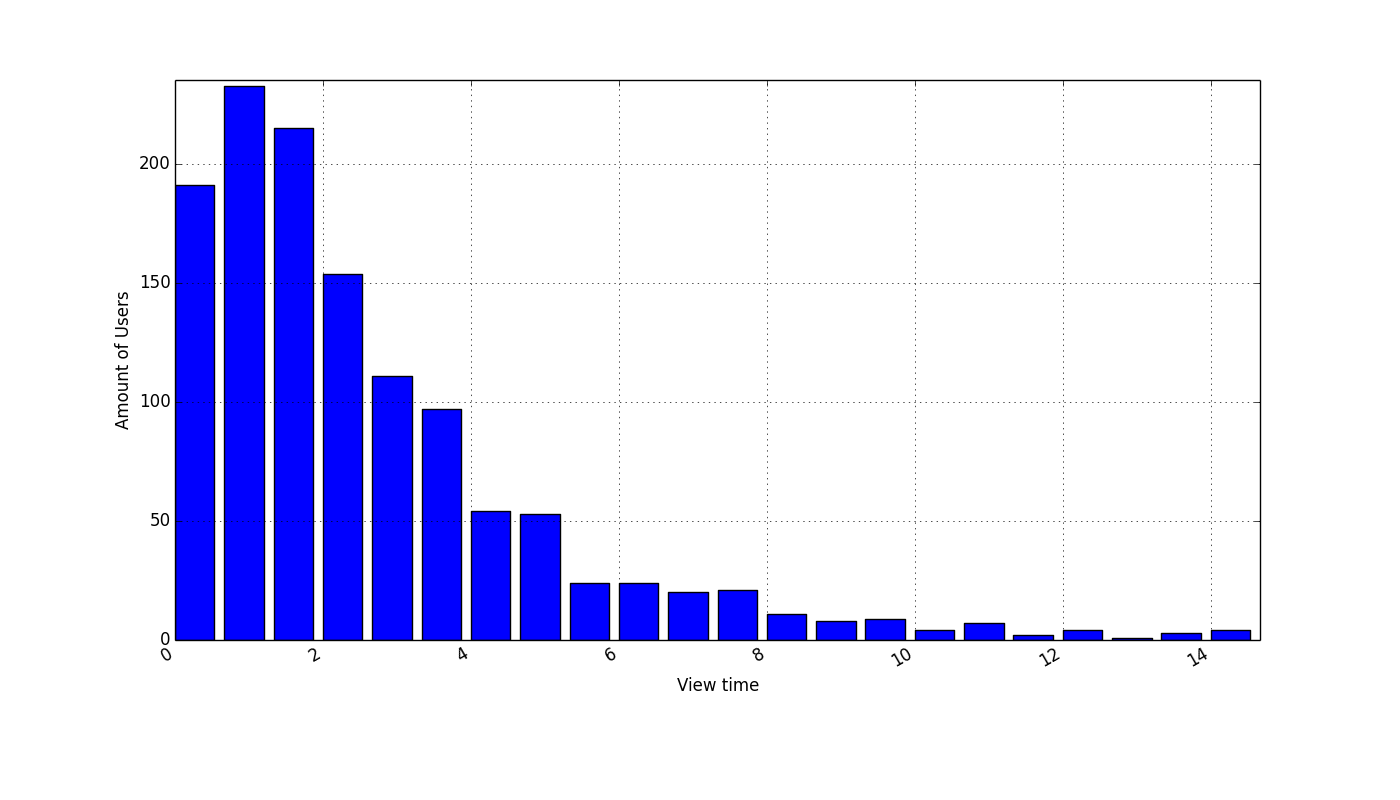
\includegraphics[width=5in]{image/product_detail_clickeddistribution.png}
        \centering
        \caption{View times before leaving an item (Bounce Rate)}
    \label{figure:bounceRate}
    \end{figure}

        This figure shows the time the users use before not taking any more action towards the item (purchase it or want it).
        The time is in milliseconds.
        The majority of the users have a view time of less than 6 000 milliseconds before they moves on to another item.

        Figure~\ref{figure:viewWant} shows the time the users use before wanting the currently viewed item.
        The time is in milliseconds.
        The majority of the users have a view time of less than 30 000 milliseconds before they want the currently viewed item.

        This figure~\ref{figure:viewBuy} shows the time the users use before purchasing the currently viewed item.
        The time is in milliseconds.
        The majority of the users have a view time of less than 32 000 milliseconds before they decide to buy the currently viewed item.

    \begin{figure}[H]
        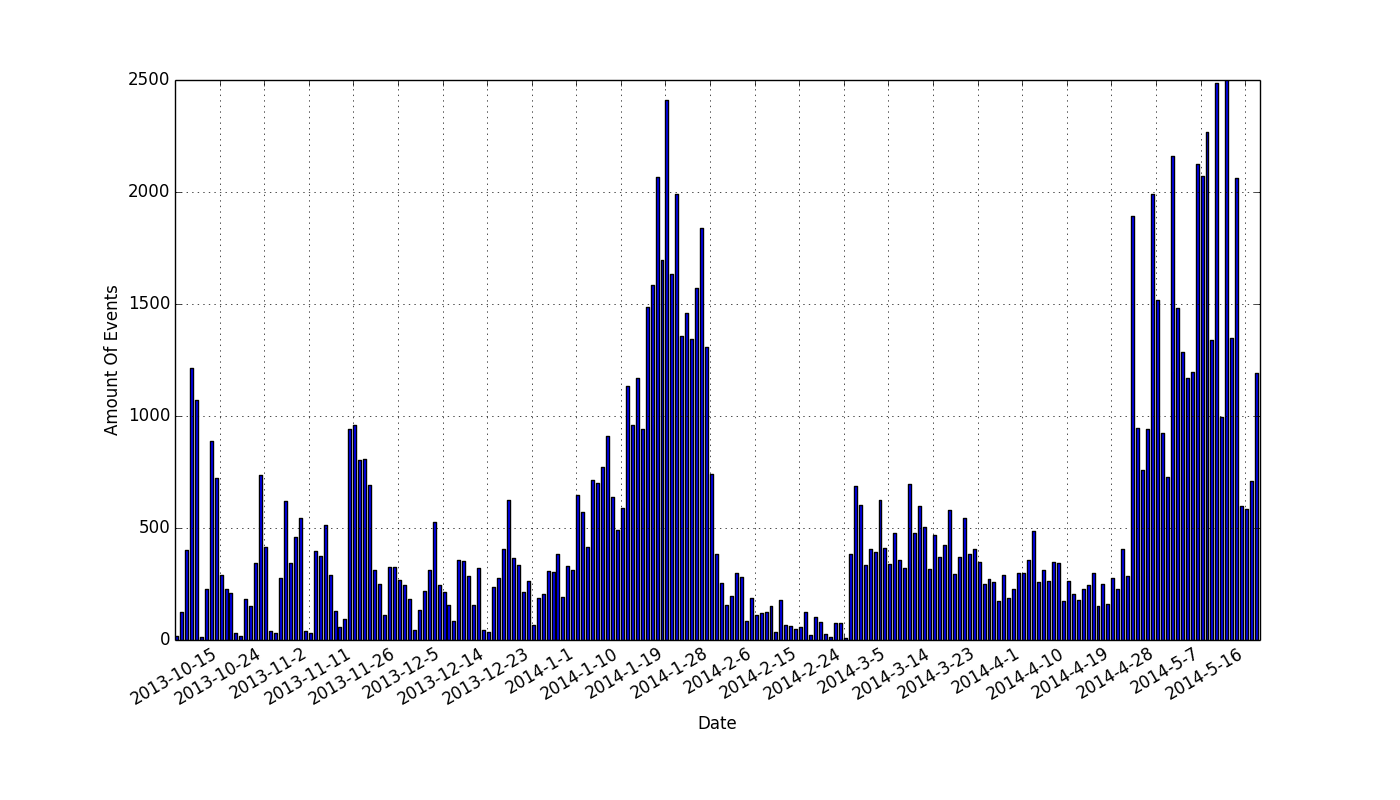
\includegraphics[width=5in]{image/eventsPerDay.png}
        \centering
        \caption{Distribution of events per day}
    \label{figure:eventOnDaysDist}
    \end{figure}
        This figure shows the event distribution per day over the time period the events were stored.
        The spikes we see happens on a weekly basis, and is centered around the weekends.
        The larger spike from the start of January to the start of March might be due to increase in publicity or other outside factors.

    \begin{figure}[H]
        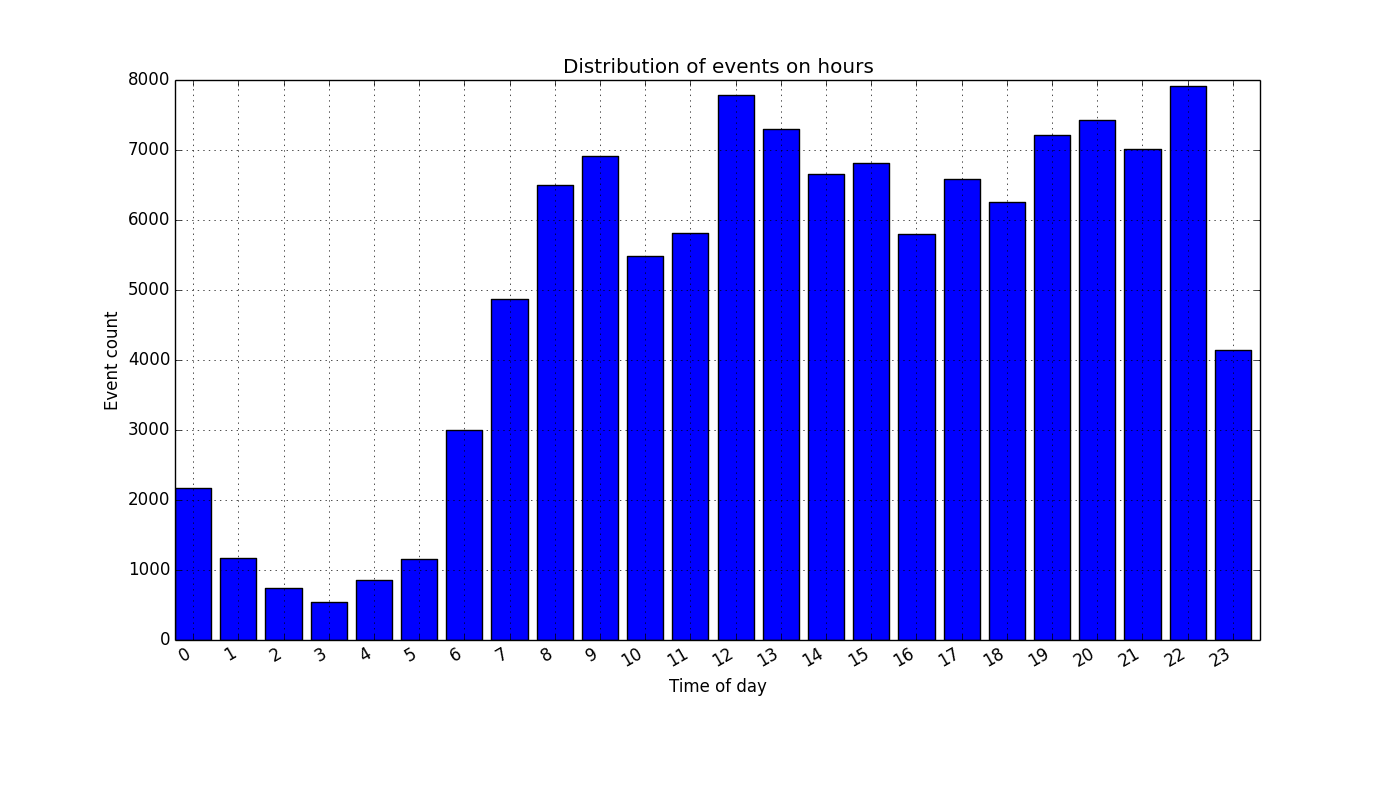
\includegraphics[width=5in]{image/hrdistribution.png}
        \centering
        \caption{mtodo}
    \label{figure:timeOfDayDistr}
    \end{figure}


\subsection{About the view time before tanking an action}
    As seen from the figures~\ref{figure:bounceRate}, ~\ref{figure:viewWant} and~\ref{figure:viewBuy}, the bounce rate is quite small compared to the time it takes for a user to decide to want or buy an item.
    This could be used as an indication of negative feedback, but since there is no explicit feedback to to test this, it might lead to rating an item negatively when the user in fact would like to rate it positively.


    %mtodo - masse fin info, men diskuter!
        % hva betyr det for oss?
        % hvordan kan data-pakket brukes av systemet?
        % dette er hands-on!
        % mange fine figurer uten konkrete beskrivelser og refereanser i teksten
        % prøv heller å lage gode forklaringer til fiugurene i teksten så referer deretter


\clearpage
\section{Conversion rate properties}

In many domains the number of activities on an item given a specific user
implies preference. The activity in question may be the number of plays in a
music service~\cite{parra2011walk} or the amount of minutes used watching a
specific TV-show~\cite{study-on-implicit-tv}. We want to validate this
hyptohesis in the SoBazaar data, determining if the \textit{number of clicks}
on an item implies higher preference, that is an higher probability of buying
the item.

\marginpar{Herman: Implicit Feedback Recommendation via Implicit-to-Explicit
Ordinal Logistic Regression Mapping
 Check out related work for similar articles}


If the hyphothesis holds true, we can use this fact in order improve
classification of our models in future sections. In addition we can customize
the user interface so that if a user has clicked the item, we should with a
higher frequency show the item to the user – as he/she is more probable of
buying it once seen in detail.

In order to validate the hyphothesis we iterate through all users and look at
their respecitive events, summarizing the number of times the user has clicked
an item $n$ times and of these how many times the user also bought it. We do
this for all values of $n$, where $n \in [1,6[$ and obtain the following table
of conversion rates and standard errors.

\begin{table}[H]
  \centering
  \begin{tabular}{lllll}
    \toprule
    N & Clicks & Purchases & Rate & Standard Error \\
    \midrule
    1 & 15602 & 1039  & 0.0667 & 0.20\% \\
    2 & 2672  & 323   & 0.1208 & 0.63\% \\
    3 & 433   & 84    & 0.1939 & 1.89\% \\
    4 & 173   & 36    & 0.2081 & 3.10\% \\
    5 & 65    & 19    & 0.2923 & 5.63\% \\
    6 & 54    & 20    & 0.3703 & 6.57\% \\
    \bottomrule
  \end{tabular}
\end{table}

The standard error gives a useful indication on how certain we can be that the
results are statisically significant, and is calculated based on the sample
size (number of clicks) and the amount of conversions. Given the rate as $r$
and sample size as $S$ we calculate the standard error $e$ as:

\begin{equation}
  e = \sqrt{\frac{r(1 - r)}{S}}
\end{equation}

Using the standard error we want to perform an hypothesis test determining if
the results are significant within our accepted confidence of 95\%. In other
words we want to be 95\% sure that the patterns found in the data are not just
random. Our two hypothesis which we want to test are thus:

$\mathbf{H_0:}$ The differences in conversion rates between our first
(baseline) and second scenerio is random.

$\mathbf{H_1:}$ The difference is significant, such that one scenario have a
higher probability of conversion.

and we want to do multiple tests when $n \in [2,6[$, using $n-1$ as baseline
and $n$ as the second scenario. For each test we calculate the
\textit{P-value}, which is the probability of obtaining a result at least as
extreme as the one that was actually observed. When the p-value becomes less
that our predetermined significance level ($0.05$ when we do a 95\%
significance test) we can reject our null-hypothesis, which is what we want to
do. In order to find this P-value we use the Standard Score, also called the
\textit{z-score}, which is the number of standard deviations an observation is
above the mean. As we have two samples we can calculate the difference in
conversion rates and use the cummulated standard error in order to find the
Z-score:

\begin{equation}
  \label{eq-z-score}
  Z = \frac{r_b - r_v}{\sqrt{e_{b}^{2} + e_{v}^{2}}}
\end{equation}

where $r_b$ and $r_v$ are the conversion rates for the baseline and second
scenario respecivly. $e_b$ and $e_v$ are equally the standard errors for the
two scenarios. Using standard normal deviate (normallly distributed random
variable with expected value 0 ($s$) and standard deviation 1 ($h$)) we can
find the cumulative probability for validity of the model - the P-value.

We calculate the P-value using $n=1$ as baseline and $n=2$ as our second
scenario. The Z-score is calculated by Equation~\ref{eq-z-score} and we obtain
our result:

\begin{equation}
  Z = \frac{0.0667-0.1208}{\sqrt{0.0020^2 + 0.0063^2}} = \frac{-0.05}{\sqrt{0.4369}} = -8.1848
\end{equation}

This is a very low Z-score, and when we are this many standard deviations away
from the mean in a standard normal deviate the P-value or area under the curve
is approximated to 0. This is a value lower than our predetermined significance
level ($0.05$) and thus we can reject the null-hypothesis and state with
statistical accuracy and correctness that there is a higher probability of
buying the item given that the user has clicked on the item twice, rather than
having clicked on the item only once. In our first scenarios we have sufficient
data to come to this conclusion, however, when comparing later scenerios we see
that our numbers stop being significant as a reult of the dataset being too
small.

\begin{table}[H]
  \centering
  \begin{tabular}{lllll}
  \toprule
  Baseline & Alternative & Z-score & P-value & Significant \\
  \midrule
  1 & 2 & -8.1848 & 0.0000 & \cmark \\
  2 & 3 & -3.6516 & 0.0001 & \cmark \\
  3 & 4 & -0.3889 & 0.3487 & \xmark \\
  4 & 5 & -1.3096 & 0.0952 & \xmark \\
  5 & 6 & -0.9013 & 0.1837 & \xmark \\
  \bottomrule
  \end{tabular}
\end{table}

Our conclusion is then that when a user has clicked on an item two times there
is a higher probability of buying it compared to when the user has only
clicked it once. This is also true when the user has clicked an item three
times, but we can not defend it statistically for any higher value of clicks.

\section{Session Findings}
\marginpar{Something about session findings perhaps}

    % mtodo - fix caption and section :P
	\marginpar{TODO: Remove all arrows with less than e.g. 50 events}
    \begin{figure}[H]
        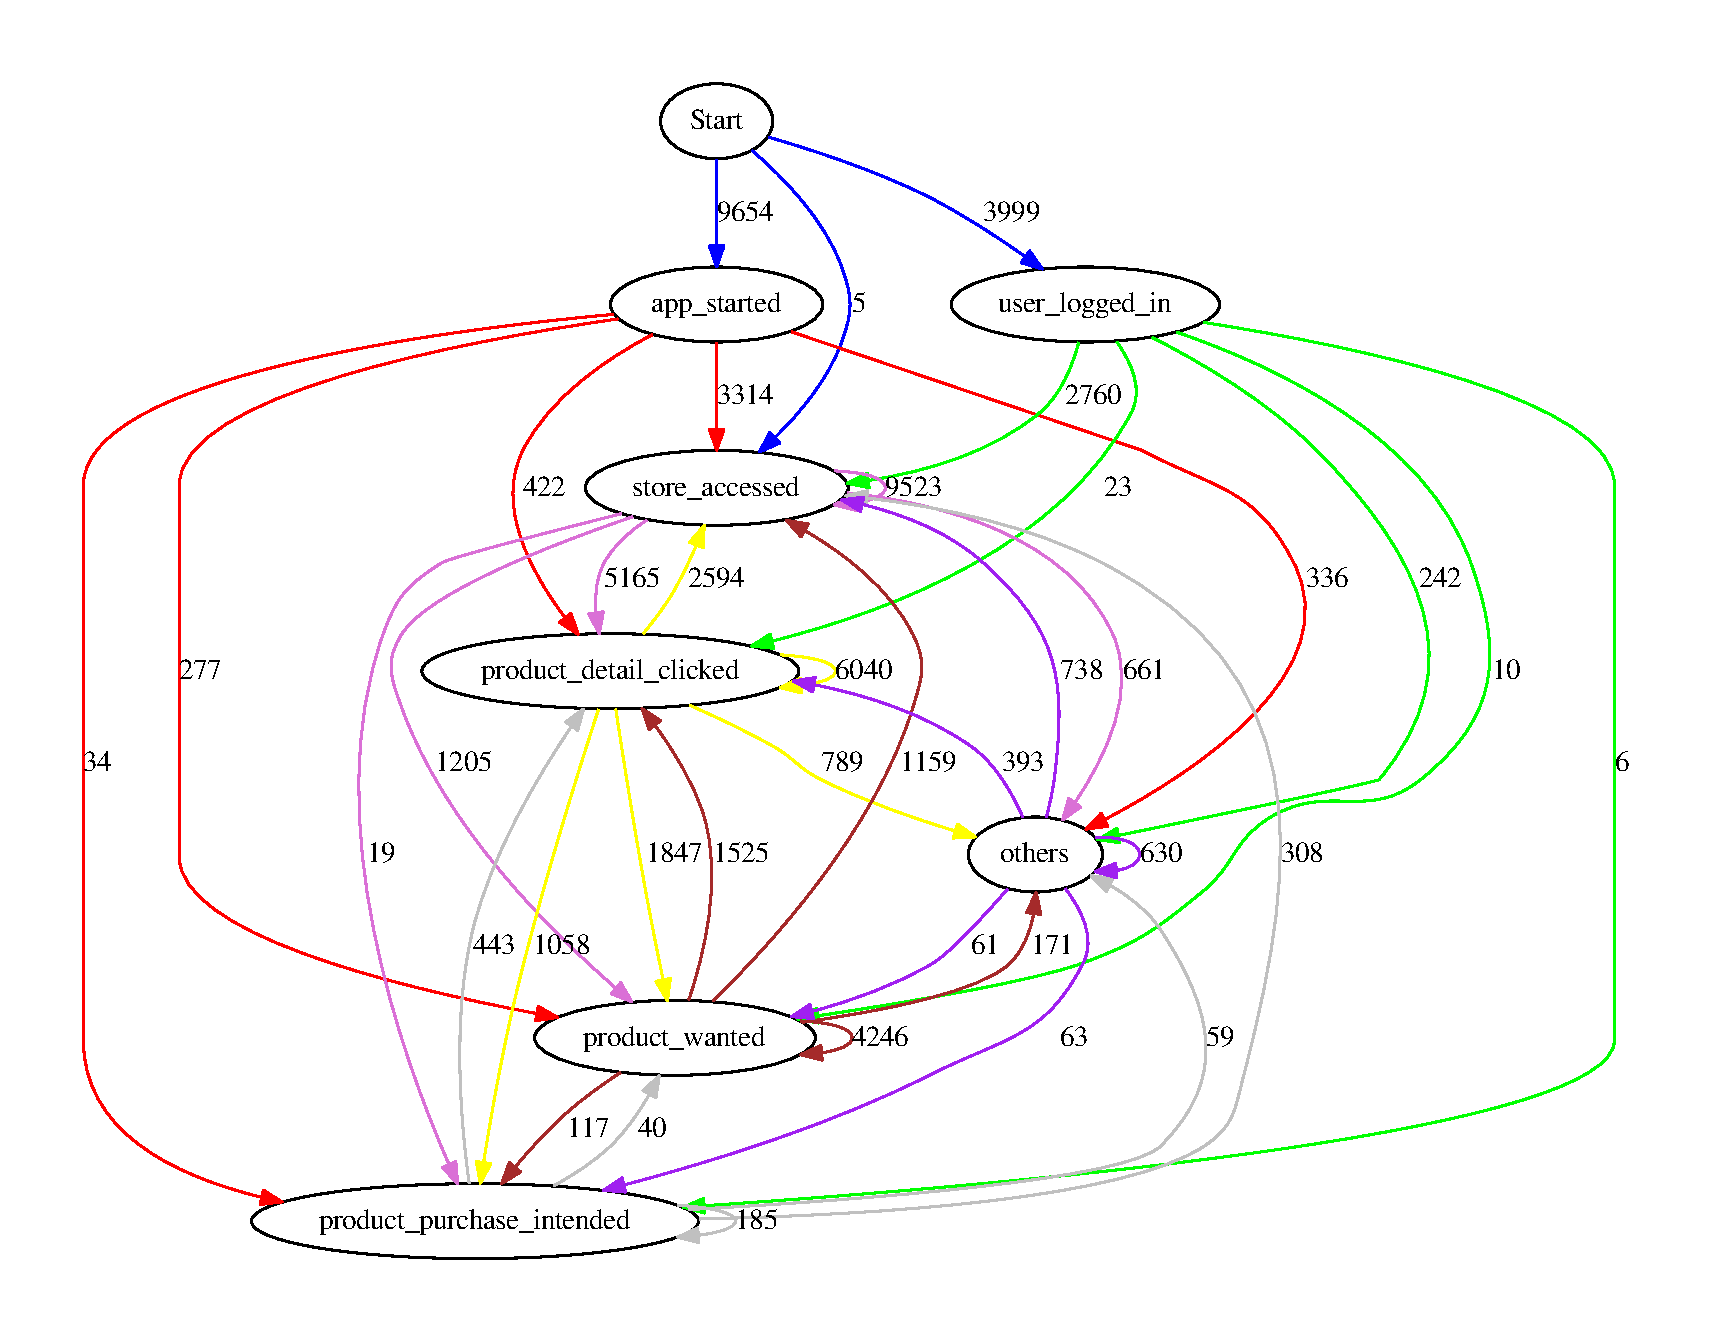
\includegraphics[width=5in]{image/statesInteractionTrue-gvfile.pdf}
        \centering
        \caption[Minimized states in session and how they interact]{A minimized view of the different states of the system and how they interact with each other.}
        \label{figure:minStatesInteractions}
    \end{figure}

    \begin{figure}[H]
        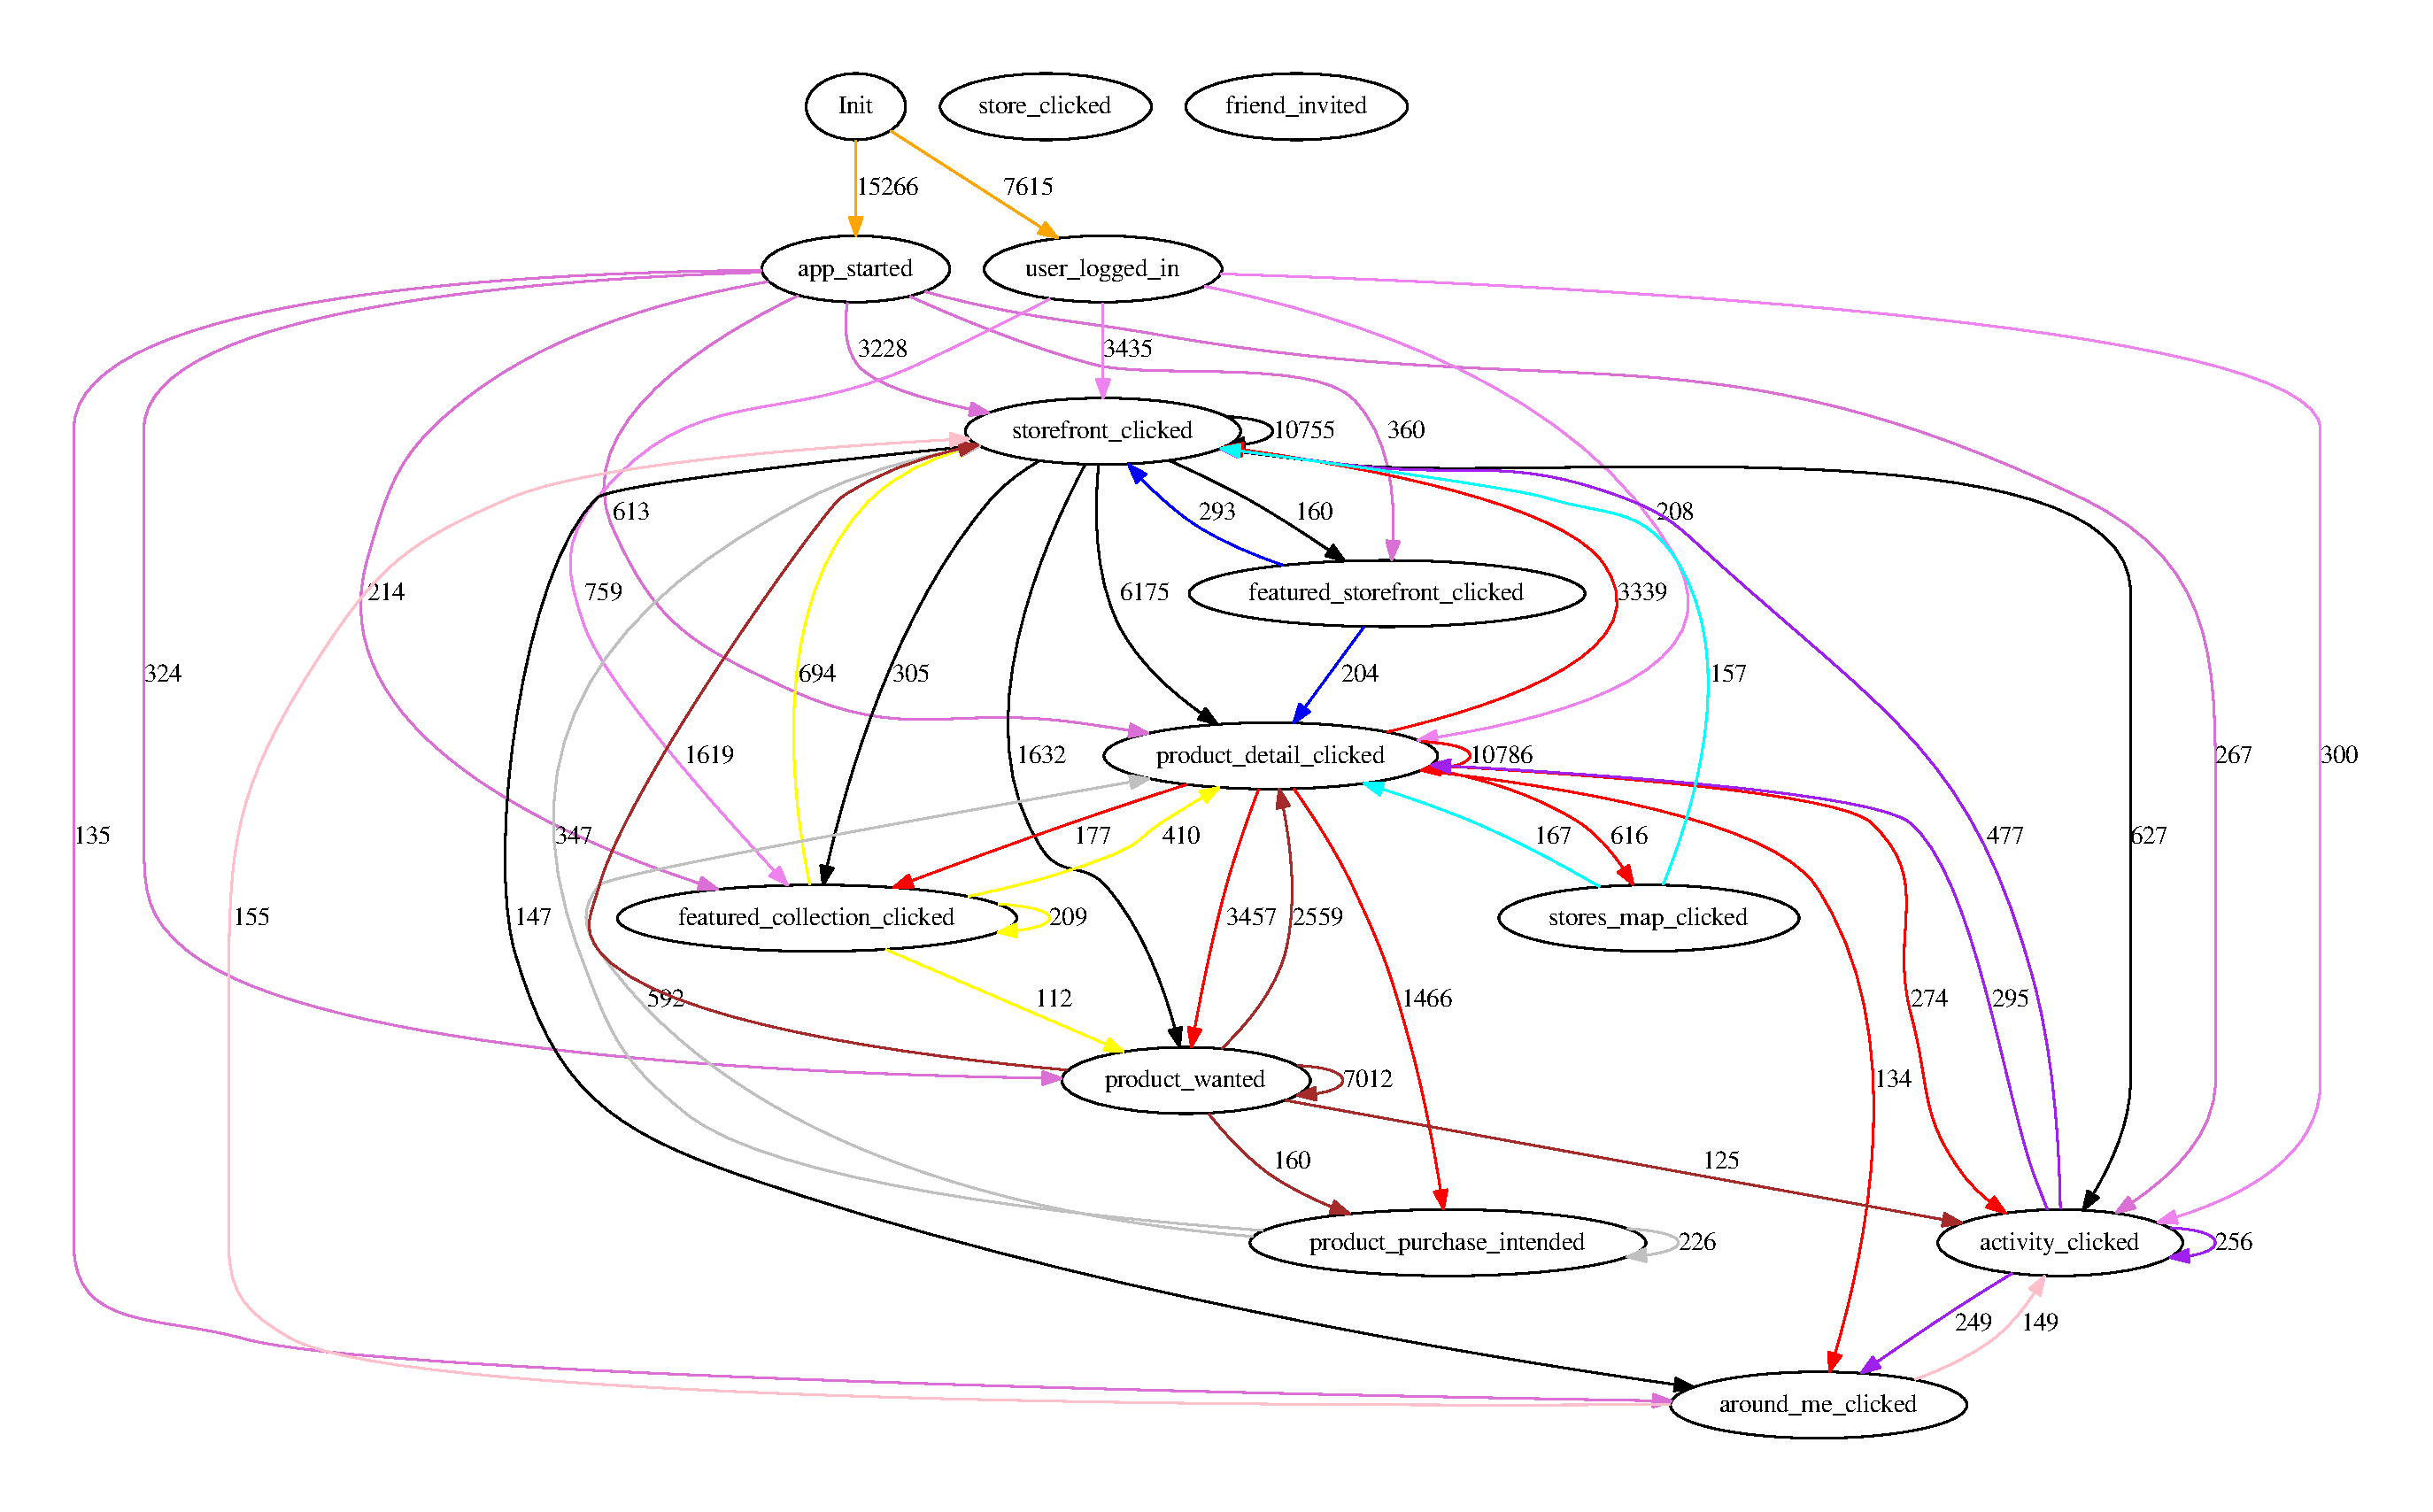
\includegraphics[width=5in]{image/statesInteractionFalse-gvfile.pdf}
        \centering
        \caption[States in session and how they interact]{The different states of the system and how they interact with each other.}
        \label{figure:statesInteractions}
    \end{figure}

    \marginpar{This is way too much information. Consider adding a threshold in
    order to reduce number of arrows}

    % mtodo - fix lol
%     Init Hypothesis:
%     Two users with similar session habits and similar product accessing pattern
%     have a stronger correlation to one-another than two users with just similar
%     product interests.


%     'product\_purchase\_intended' (user pushed to the product web store) shows a
%     wider specter of information about the product, including additional colors,
%     images and colors.  For some it might be natural to explore the item there
%     before "wanting" it. Making both

%     "product\_purchase\_intended" $\Rightarrow$ "product\_wanted"

%     and

%     "product\_purchase\_intended" $\notimplies$ "product\_wanted"

%     produce valuable information.

%     Must make different rules for the different stores:
%     "Bik Bok", "Cubus", "Gina Trik", "H\&M", "Bianco" has a broad specter of extra
%     functions inside the web store, whereas others might not, only shows the
%     product and a add to chart button.  This might divide the use pattern of the
%     users into a:

%     "product\_detail\_clicked" $\Rightarrow$ "product\_purchase\_intended" $\Rightarrow$ "product\_wanted"

%     "product\_detail\_clicked" $\Rightarrow$ "product\_purchase\_intended" $\notimplies$ "product\_wanted",

%     and

%     "product\_detail\_clicked" $\Rightarrow$ "product\_wanted"

%     based on the store accessed.

%     Use this to make a "rule set" with a probability.
%     Then again use this to recommend items for the users with that given
%     probability.

%     Find a "most popular session"-pattern
%     Find a "most likely to come after"-pattern

%     Session issues:
%     Once in a blue moon a user will do a "product action" (purchase,want,details)
%     without having a previous frontstore-access event. Which leads to unknown
%     store-id of the item.

%     Issue is most probably from missing user-id in collection\_viewed, and a user
%     checks out an item from there. It is not possible to be 100\% sure which user
%     access the item from the collection\_viewed event, so this event is therefor
%     not integrated into the session-stack.


\section{Conclusion}

%Summarize the findings
%What can be used?

